% \setcounter{section}{0}% Change the chapter counter value
% %\numberwithin{equation}{chapter}% Equation counter follows chapter
% \numberwithin{equation}{section}% Equation counter follows section
% \numberwithin{figure}{chapter}% Figure counter follows chapter
% \setcounter{chapter}{1}

\chapter{\texorpdfstring{Conformal field theory}{2 Conformal field theory}} \label{cha:2}

\section{\texorpdfstring{Massless scalars in two dimensions}{2.1 Massless scalars in two dimensions}} \label{sec:2.1}
We start from $D$ free scalar fields $X^{\mu}(\sigma^{1}, \sigma^{2})$ in two dimensions. In anticipation of application to string theory, we call this two-dimensional space the worldsheet.    
The action is    
\begin{equation}
	S=\frac{1}{4 \pi \alpha^{\prime}} \int \dif^{2} \: \sigma
	\Bigl(\partial_{1} X^{\mu} \partial_{1} X_{\mu}+\partial_{2} X^{\mu} \partial_{2} X_{\mu}\Bigr) \:. \label{2.1.1}
\end{equation}
This is the Polyakov action (\ref{1.2.13}) where the worldsheet metric $\gamma_{a b}$ is taken to be the flat Euclidean metric $\delta_{a b}$, with signature $(+,+)$.    
Most string theory calculations will be performed on the Euclidean worldsheet.    
At least for flat metrics, the relationship between Euclidean amplitudes and Minkowski amplitudes is given by standard analytic continuation.    
We will use the Minkowski flat metric for the index $\mu$.    

Canonical quantization of the action (\ref{2.1.1}) is straightforward: finding the spectrum, vacuum expectation values, and so on. What we did in Chapter 1 was to complete these in the light-cone gauge.    
Here we will take a different route, first studying various local properties, such as equations of motion, operator products, Ward identities, and conformal invariance, and only then the spectrum.    
We will use the more effective path integral formalism. We will primarily use path integral representations to derive operator equations; these equations can also be obtained in the Hilbert space formalism.    
Adopting complex coordinates    
\begin{equation}
	z=\sigma^{1}+ \mi \sigma^{2} \:, \qquad \bar{z}=\sigma^{1}- \mi \sigma^{2} \label{2.1.2}
\end{equation}
is very convenient. We will use a bar to represent the conjugate of $z$ and other complex variables, and for longer expressions, an asterisk. Also define    
\begin{equation}
	\partial_{z}=\frac{1}{2}(\partial_{1}- \mi \partial_{2}) \:, \qquad \partial_{\bar{z}}=\frac{1}{2}(\partial_{1}+ \mi \partial_{2}) \:.
	\label{2.1.3}
\end{equation}
These variables satisfy    
\begin{equation}
	\partial_{z} z=1 \:, \quad \partial_{z} \bar{z}=0 \:, \quad \partial_{\bar{z}} z=0 \:, \quad \partial_{\bar{z}} \bar{z}=1
	\:. \label{2.1.4}
\end{equation}
When there is no ambiguity, $\partial_{z}$ is abbreviated as $\partial$ and $\partial_{\bar{z}}$ as $\bar{\partial}$.    
For a general vector $v^{a}$, define in the same way    
\begin{equation}
	v^{z}=v^{1}+ \mi v^{2} \:, \quad v^{\bar{z}}=v^{1}- \mi v^{2} \:, \quad v_{z}=\frac{1}{2}(v^{1}-\mi v^{2}) \:, \quad v_{\bar{z}}=\frac{1}{2}(v^{1}+ \mi v^{2}) \:.
	\label{2.1.5}
\end{equation}
For complex indices, raising and lowering indices is accomplished via    
\begin{equation}
	g_{z \bar{z}}=g_{\bar{z} z}=\frac{1}{2} \:, \quad g_{z z}=g_{\bar{z} \bar{z}}=0 \:, \quad g^{z \bar{z}}=g_{\bar{z} z}=2 \:, \quad g^{z z}=g^{\bar{z} \bar{z}}=0
\end{equation}
In matrix form:
\begin{equation}\label{matrix-metric}
	g_{ab} = 
	\bordermatrix{
		& \textcolor{gray}{z} & \textcolor{gray}{\bar{z}} \cr
		\textcolor{gray}{z} & 0 & 1/2 \cr
		\textcolor{gray}{\bar{z}} & 1/2 & 0 \cr
	}
\end{equation}
Also note    
\begin{equation}
	\dif^{2} z=2 \dif \sigma^{1} \dif \sigma^{2}
\end{equation}
The factor 2 comes from the Jacobian, $\dif^{2} z\, \lvert \operatorname{det} g\rvert^{1/2}= \dif \sigma^{1} \dif \sigma^{2}$.    
We define    
\begin{equation}
	\int \dif^{2} z \: \delta^{2}(z, \bar{z})=1 \:,
\end{equation}
so that $\delta^{2}(z, \bar{z})=\tfrac{1}{2} \delta(\sigma^{1}) \delta(\sigma^{2})$.    
The divergence formula in complex coordinates is    
\begin{equation}
	\int_{R} \dif^{2}z\: (\partial_{z} v^{z}+\partial_{\bar{z}} v^{\bar{z}} )= \mi \oint_{\partial R}\: (v^{z} \dif \bar{z}-v^{\bar{z}} \dif z ) \:, \label{2.1.9}
\end{equation}
where the integration contour runs counterclockwise around the boundary of the region $R$.    
In this sign convention, the action is    
\begin{equation}
	S=\frac{1}{2 \pi \alpha^{\prime}} \int 2\dif^{2} \sigma\frac{\partial_1 X^{\mu}\partial_1 X_{\mu}+\partial_2X^{\mu}\partial_2X_{\mu}}{4}=\frac{1}{2 \pi \alpha^{\prime}} \int \dif^{2} z\: \partial X^{\mu} \bar{\partial} X_{\mu} \:, \label{2.1.10}
\end{equation}
The classical equations of motion are    
\begin{equation}\
	\frac{\delta S}{\delta X_{\mu}(z, \bar{z})}=0\implies\partial \bar{\partial} X^{\mu}(z, \bar{z})=0 \:. \label{2.1.11}
\end{equation}
Here $f(z)$ refers to those functions that are analytic (equivalently, holomorphic) in $z$.    
Writing the equations of motion as    
\begin{equation}
	\partial(\bar{\partial} X^{\mu})=\bar{\partial}(\partial X^{\mu})=0 \:, \label{2.1.12}
\end{equation}
it follows that $\partial X^{\mu}$ is holomorphic and $\bar{\partial} X^{\mu}$ is anti-holomorphic (holomorphic in $\bar{z}$), thus we have $\partial X^{\mu}(z)$ and $\bar{\partial} X^{\mu}(\bar{z})$.    

Under the Minkowski continuation $\sigma^{2}=\mi \sigma^{0}$, the holomorphic field becomes a function of $\sigma^{0}-\sigma^{1}$, while the anti-holomorphic field becomes a function of $\sigma^{0}+\sigma^{1}$.    
Thus there is the following correspondence:    
\begin{subequations}
	\begin{align}
		{\text{holomorphic}}&=\text {left-moving}  \:,\\
		{\text{anti-holomorphic}}&=\text {right-moving} \:.
	\end{align}
\end{subequations}


Vacuum expectation values are defined by path integrals,    
\begin{equation}
	\langle\mathscr{F}[X]\rangle=\int[\dif X]\: \exp (-S) \mathscr{F}[X] \:,
\end{equation}
where $\mathscr{F}[X]$ is any functional of $X$, for example a product of local operators. In order for the path integral over $X^{0}$ to be a convergent Gaussian integral, it is defined through analytic continuation $X^{0} \to -\mi X^{D}$. We do not normalize $\langle\mathscr{F}[X]\rangle$ by dividing by $\langle 1\rangle$.    
The path integral of a total derivative is zero. Then,    
\begin{align}
	0 &=\int[\dif X]\: \frac{\delta}{\delta X_{\mu}(z, \bar{z})} \exp (-S) \nonumber \\
	&=-\int[\dif X]\: \exp (-S) \frac{\delta S}{\delta X_{\mu}(z, \bar{z})} \nonumber  \\
	&=-\left\langle\frac{\delta S}{\delta X_{\mu}(z, \bar{z})}\right\rangle  \tag{can be simplified using \eqref{2.1.11}} \\
	&=\frac{1}{\pi \alpha^{\prime}}\Bigl\langle\partial \bar{\partial} X^{\mu}(z, \bar{z})\Bigr\rangle \:.
	\label{2.1.15}
\end{align}
If we have additional arbitrary insertions "$\cdots$" in the path integral, the calculation is the same as long as those additional operators are not inserted at $z$. Therefore    
\begin{equation}
	\Bigl\langle\partial \bar{\partial} X^{\mu}(z, \bar{z}) \cdots\Bigr\rangle=0 \:. \label{2.1.16}
\end{equation}
We can view the additional insertions as preparing arbitrary initial and final states (we can do the same thing for situations with boundary conditions).    
The path integral formula (\ref{2.1.16}) thus corresponds to the operator equation    
\begin{equation}
	\partial \bar{\partial} \hat{X}^{\mu}(z, \bar{z})=0 \label{2.1.17}
\end{equation}
which holds for all matrix elements of the operator $\hat{X}^{\mu}(z, \bar{z})$ in the Hilbert space formalism. Therefore we call the relationship established in the sense of (\ref{2.1.16}) an operator equation. The equation (\ref{2.1.17}) is the Ehrenfest theorem translating the classical equations of motion into operator equations.    

The notation "$\cdots$" in the path integral (\ref{2.1.16}) implies that the insertions are away from $z$.    
Now consider the case where the insertion is exactly at $z$:    
\begin{align}
	0 &=\int[\dif X] \: \frac{\delta}{\delta X_{\mu}(z, \bar{z})}\Bigl[\exp (-S) X^{v}(z^{\prime}, \bar{z}^{\prime})\Bigr] \nonumber \\
	&=\int[\dif X]\: \exp (-S)\left[\eta^{\mu v} \delta^{2}(z-z^{\prime}, \bar{z}-\bar{z}^{\prime})+\frac{1}{\pi \alpha^{\prime}} \partial_{z} \partial_{\bar{z}} X^{\mu}(z, \bar{z}) X^{v}(z^{\prime}, \bar{z}^{\prime})\right] \nonumber \\
	&=\eta^{\mu v}\left\langle\delta^{2}(z-z^{\prime}, \bar{z}-\bar{z}^{\prime})\right\rangle+\frac{1}{\pi \alpha^{\prime}} \partial_{z} \partial_{\bar{z}}\left\langle X^{\mu}(z, \bar{z}) X^{v}(z^{\prime}, \bar{z}^{\prime})\right\rangle \label{2.1.18}
\end{align}
That is, the equation of motion holds outside of the coincidence point.
\begin{tcolorbox}[breakable]
	\begin{remark}These are all special case of the Schwinger Dyson Equation. To derive it, we start with the path integral expectation value:
			\begin{equation}
				\langle \mathscr{F}[X] \rangle 
				= \int \mathcal{D}X \, \mathscr{F}[X] \, e^{-S[X]}.
			\end{equation}
			
			Now consider the functional total derivative:
			\begin{equation}
				0 = \int \mathcal{D}X \, 
				\frac{\delta}{\delta X^\mu(\sigma)} 
				\Big( \mathscr{F}[X] \, e^{-S[X]} \Big).
			\end{equation}
			
			Expanding using the product rule:
			\begin{equation}
				0 = \int \mathcal{D}X \left[
				\frac{\delta \mathscr{F}}{\delta X^\mu(\sigma)} 
				- \mathscr{F} \frac{\delta S}{\delta X^\mu(\sigma)}
				\right] e^{-S[X]}.
			\end{equation}
			
			Dividing by the partition function, we obtain:
			\begin{equation}
				\left\langle \frac{\delta \mathscr{F}}{\delta X^\mu(\sigma)} \right\rangle
				=
				\left\langle \frac{\delta S}{\delta X^\mu(\sigma)} \, \mathscr{F} \right\rangle.\label{impiden}
			\end{equation}
			Therefore in general case this is proportional to $\delta(\sigma-\sigma')$.
	\end{remark}
\end{tcolorbox}
Inserting "$\cdots$" in the path integral once more:    
\begin{equation}
	\frac{1}{\pi \alpha^{\prime}} \partial_{z} \partial_{\bar{z}}\left\langle X^{\mu}(z, \bar{z}) X^{v}(z^{\prime}, \bar{z}^{\prime}) \cdots\right\rangle=-\eta^{\mu \nu}\left\langle\delta^{2}(z-z^{\prime}, \bar{z}-\bar{z}^{\prime}) \cdots\right\rangle
\end{equation}
thus    
\begin{equation}
	\frac{1}{\pi \alpha^{\prime}} \partial_{z} \partial_{\bar{z}} X^{\mu}(z, \bar{z}) X^{v}(z^{\prime}, \bar{z}^{\prime})=-\eta^{\mu v} \delta^{2}(z-z^{\prime}, \bar{z}-\bar{z}^{\prime}) \label{2.1.20}
\end{equation}
holds as an operator equation.    
In the Hilbert space formalism, the products in the path integral appear as time-ordered products, and the $\delta$-function comes from derivatives acting on the time-ordered product. This connection is further developed in the appendix.    

In free field theory, it is useful to introduce normal-ordered operators. The normal-ordering of an operator is denoted as $:\mathrel{\mathscr{A}}:$, defined as follows:    
\begin{subequations} \label{2.1.21}
	\begin{align}
		: \mathrel{X^{\mu}(z, \bar{z})}:&=X^{\mu}(z, \bar{z}) :, \label{2.1.21a}\\
		: \mathrel{X^{\mu}(z_{1}, \bar{z}_{1}) X^{v}(z_{2}, \bar{z}_{2})}:&=X^{\mu}\left(z_{1}, \bar{z}_{1}\right) X^{v}(z_{2}, \bar{z}_{2})+\frac{\alpha^{\prime}}{2} \eta^{\mu v} \ln \lvert z_{12}\rvert^{2} \:, \label{2.1.21b}
	\end{align}
\end{subequations}
where    
\begin{equation}
	z_{i j}=z_{i}-z_{j}
\end{equation}
\begin{tcolorbox}[breakable]
	The mode function for closed string \eqref{2.7.4} with $w=\sigma^1+i\sigma^2$ (refer \eqref{2.6.3}) can be given as:
	\begin{equation}\label{mode-expansion-boson} 
		X^{\mu}(w,\overline{w}) = x^{\mu}-i\frac{\alpha'}{2} p^{\mu} (w+\overline{w})+i\sqrt{\frac{\alpha'}{2}}\sum_{n\neq 0} \frac{1}{n} \bigg( \alpha^{\mu}_n e^{-2\pi n w /L} + \overline{\alpha}^{\mu}_n e^{-2\pi n\overline{w})/L}
		\bigg)\, ,
	\end{equation}
	with now $w\sim w+iL$. Using a conformal transformation, we map all the operators from the cylinder  to the complex plane:
	$$z=e^{2\pi w /L}\, , \qquad   \overline{z}=e^{2\pi \overline{w}/L}$$
	we finally obtain the expansion by simply replacing $w$ by $z$.
	\begin{equation}   X^{\mu}(z, \overline{z})  =x^{\mu}-i\frac{\alpha'}{2} p^{\mu} \ln(z\overline{z})  +i\sqrt{\frac{\alpha'}{2}}\sum_{n\neq 0} \frac{1}{n}   (\alpha^{\mu}_n z^{-n}+\overline{\alpha}^{\mu}_n \overline{z}^{-n}  )\, . \end{equation}
	The propagator could be calculated by assuming $|z|>|z'|$ and considering the product
	
	\begin{multline*}
		X^{\mu}(z,\bar z)\,X^{\mu}(z',\bar z')
		\;=\;
		\Big[x^{\mu}-i\frac{\alpha'}{2} p^{\mu} \ln|z|^2  + i\sqrt{\frac{\alpha'}{2}}\sum_{m\neq0}\frac{1}{m}(\alpha^{\mu}_m z^{-m}+\overline \alpha^{\mu}_m\bar z^{-m})\Big]\\
		\qquad\qquad\times
		\Big[x^{\mu}-i\frac{\alpha'}{2} p^{\mu} \ln|z'|^2  +  i\sqrt{\frac{\alpha'}{2}}\sum_{n\neq0}\frac{1}{n}(\alpha^{\mu}_n z'^{-n}+\overline \alpha^{\mu}_n\bar z'^{-n})\Big].
	\end{multline*}
	We will move annihilation operators ($a_k,\overline a_k$ with $k>0$) and $\pi_0$ to the right to reach normal ordering; non-vanishing c-number contributions come from $[x^{\mu},p^{\nu}]=i\eta^{\mu\nu}$ and $[\alpha^{\mu}_m,\alpha^{\nu}_n]=m\eta^{\mu\nu}\delta_{m+n,0}$, $[\overline \alpha^{\mu}_m,\overline \alpha^{\mu}_n]=m\eta^{\mu \nu}\delta_{m+n,0}$. Let's first focus on these terms
	\begin{align*}
		\Big(x^{\mu}-&i\frac{\alpha'}{2} p^{\mu} \ln|z|^2 \Big)\Big(x^{\nu}-i\frac{\alpha'}{2} p^{\nu} \ln|z'|^2\Big)\\
		&= x^\mu x^\nu
		-i\frac{\alpha'}{2}x^\mu p^\nu \ln|z'|^2
		-i\frac{\alpha'}{2}p^\mu x^\nu \ln|z|^2
		-\Big(\frac{\alpha'}{2}\Big)^2 p^\mu p^\nu \ln|z|^2\ln|z'|^2\\
		&= x^\mu x^\nu
		-i\frac{\alpha'}{2}x^\mu p^\nu \ln|z'|^2
		-i\frac{\alpha'}{2}\big(x^\nu p^\mu - i\eta^{\mu\nu}\big)\ln|z|^2
		-\Big(\frac{\alpha'}{2}\Big)^2 p^\mu p^\nu \ln|z|^2\ln|z'|^2\\
		&= x^\mu x^\nu
		-i\frac{\alpha'}{2}x^\mu p^\nu \ln|z'|^2
		-i\frac{\alpha'}{2}x^\nu p^\mu \ln|z|^2
		-\Big(\frac{\alpha'}{2}\Big)^2 p^\mu p^\nu \ln|z|^2\ln|z'|^2
		-\frac{\alpha'}{2}\eta^{\mu\nu}\ln|z|^2\\
		&=\underbrace{x^\mu x^\nu
			-i\frac{\alpha'}{2}x^\mu p^\nu \ln|z'|^2
			-i\frac{\alpha'}{2}x^\nu p^\mu \ln|z|^2
			-\Big(\frac{\alpha'}{2}\Big)^2 p^\mu p^\nu \ln|z|^2\ln|z'|^2}_{\text{normal ordered}}
		-\frac{\alpha'}{2}\eta^{\mu\nu}\ln|z|^2\\
		&=\,:\!\Big(x^{\mu}-i\frac{\alpha'}{2} p^{\mu} \ln|z|^2 \Big)\Big(x^{\nu}-i\frac{\alpha'}{2} p^{\nu} \ln|z'|^2 \Big)\!:
		\;-\;\frac{\alpha'}{2}\eta^{\mu\nu}\ln|z|^2.
	\end{align*}
	The zero-mode reordering produces the c-number $-\frac{\alpha'}{2}\eta^{\mu\nu}\ln|z|^2$. Next, we'll consider holomorphic oscillator pieces
	$$
	i\sqrt{\frac{\alpha'}{2}}\sum_{m\neq0}\frac{1}{m}\alpha^{\mu}_m z^{-m}
	\quad\text{and}\quad
	i\sqrt{\frac{\alpha'}{2}}\sum_{n\neq0}\frac{1}{n}\alpha^{\mu}_n z'^{-n}.
	$$
	We can split the sum in two parts,
	$$
	\sum_{m\neq0}\frac{1}{m}\alpha^{\mu}_m z^{-m}
	=\sum_{m=-\infty}^{-1}\frac{1}{m}\alpha^{\mu}_m z^{-m}+\sum_{m=1}^{\infty}\frac{1}{m}\alpha^{\mu}_m z^{-m}.
	$$
	The only non-normal-ordered combination producing a c-number is the product of the $m>0$ part from the first bracket with the $n<0$ part from the second bracket. That term is
	
	$$
	\Big(i\sqrt{\frac{\alpha'}{2}}\Big)^2
	\Big(\sum_{m=1}^{\infty}\frac{1}{m}\alpha^{\mu}_m z^{-m}\Big)
	\Big(\sum_{n=-\infty}^{-1}\frac{1}{n}\alpha^{\nu}_n z'^{-n}\Big)
	= -\frac{\alpha'}{2}\sum_{m=1}^\infty\sum_{n=-\infty}^{-1}\frac{1}{mn}\,\alpha^{\mu}_m \alpha^{\nu}_n\,z^{-m}z'^{-n}.
	$$
	Using $\alpha^{\mu}_m \alpha^{\nu}_n = :\!\alpha^{\mu}_n \alpha^{\nu}_m\!:+[\alpha^{\mu}_m,\alpha^{\nu}_n]=:\!\alpha^{\mu}_n \alpha^{\nu}_m\!:+m\eta^{\mu \nu}\delta_{m+n,0}$. The only contributing commutator in the sum over $n$ occurs when $n=-m$. Isolating that, we have:
	
	$$
	-\frac{\alpha'}{2}\sum_{m=1}^\infty\frac{1}{m(-m)}\;m\;z^{-m}z'^{m}
	= -\frac{\alpha'}{2}\sum_{m=1}^\infty\frac{-1}{m}\Big(\frac{z'}{z}\Big)^m
	= \frac{\alpha'}{2}\sum_{m=1}^\infty\frac{1}{m}\Big(\frac{z'}{z}\Big)^m.
	$$
	Thus the holomorphic oscillators give the c-number
	
	$$
	\boxed{\;\frac{\alpha'}{2}\sum_{m=1}^\infty\frac{1}{m}\Big(\frac{z'}{z}\Big)^m\;}.
	$$
	By identical steps for $\overline a_m$ modes we obtain
	
	$$
	\boxed{\;\frac{\alpha'}{2}\sum_{m=1}^\infty\frac{1}{m}\Big(\frac{\bar z'}{\bar z}\Big)^m\; }.
	$$
	Collecting the zero-mode, holomorphic and anti-holomorphic c-number contributions:
	
	$$
	-\frac{\alpha'}{2}\ln|z|^2
	\;+\;\frac{\alpha'}{2}\sum_{m=1}^\infty\frac{1}{m}\Big(\frac{z'}{z}\Big)^m
	\;+\;\frac{\alpha'}{2}\sum_{m=1}^\infty\frac{1}{m}\Big(\frac{\bar z'}{\bar z}\Big)^m.
	$$
	We can use $-\ln(1-x)=\sum_{m=1}^\infty x^m/m$ to simplify the series expansion (valid for $|z'|<|z|$):
	
	$$
	\sum_{m=1}^\infty\frac{1}{m}\Big(\frac{z'}{z}\Big)^m = -\ln\Big(1-\frac{z'}{z}\Big),
	\qquad
	\sum_{m=1}^\infty\frac{1}{m}\Big(\frac{\bar z'}{\bar z}\Big)^m = -\ln\Big(1-\frac{\bar z'}{\bar z}\Big).
	$$
	So the total c-number becomes
	$$
	-\frac{\alpha'}{2}\ln|z|^2 \;-\;\frac{\alpha'}{2}\ln\Big|1-\frac{z'}{z}\Big|^2
	= -\frac{\alpha'}{2}\ln\Big| z\Big(1-\frac{z'}{z}\Big)\Big|^2
	= -\frac{\alpha'}{2}\ln|z-z'|^2.
	$$
	Therefore
	
	$$\boxed{X^{\mu}(z,\bar z)X^{\nu}(z',\bar z')
		= :X^{\mu}(z,\bar z)X^{\nu}(z',\bar z'):
		- \frac{\alpha'}{2}\eta^{\mu \nu}\,\ln|z-z'|^2}$$
		
\end{tcolorbox}
Readers may be familiar with the normal ordering defined by raising and lowering operators.    
These two definitions will be connected later.    
The key point of this definition is the property:    
\begin{equation}
	\partial_{1} \bar{\partial}_{1}\!\!:\mathrel{X^{\mu}(z_{1}, \bar{z}_{1}) X^{v}(z_{2}, \bar{z}_{2})}:=0 \label{2.1.23}
\end{equation}
The above comes from the operator equation (\ref{2.1.20}) and the following differential equation:    
\begin{equation}
	\partial \bar{\partial} \ln |z|^{2}=2 \pi \delta^{2}(z, \bar{z})\label{2.1.24}
\end{equation}
Since $\ln |z|^{2}=\ln z+\ln \bar{z}$, the above equation is obvious for $z \neq 0$.    
The normalization of the $\delta$-function can be easily verified by integrating both sides using (\ref{2.1.9}).    
\begin{tcolorbox}[breakable]
	\begin{proof}
		Using \eqref{2.1.9}, we can write
		\begin{align}
			\frac{1}{2\pi} \int_M d^2z \, f(z) \, \partial_{\bar z} \frac{1}{z}
			&= \frac{1}{2\pi} \int_M d^2z \, \partial_{\bar z} \left( \frac{f(z)}{z} \right) \notag \\
			&= \frac{1}{2\pi i} \int_{\partial M} dz \, \frac{f(z)}{z} \notag \\
			&= f(0)
		\end{align}
		Alternatively,
		\begin{align*}
			\pdv{z}\left(\frac{1}{\bar z}\right)=\partial_z\lim\limits_{\epsilon\to0}\frac{z}{|z|^2+\epsilon^2}=\lim_{\epsilon\to0}\frac{\epsilon^2}{(|z|^2+\epsilon^2)^2}=2\pi\delta^2(z)
		\end{align*}
		The extra factor of $2$ is here because of the way we defined our integration measure. It's a choice of normalization that we're adopting.
	\end{proof}
\end{tcolorbox}
\section{\texorpdfstring{The operator product expansion}{2.2 The operator product expansion}}

\begin{figure}[!htbp]
	\begin{center}
		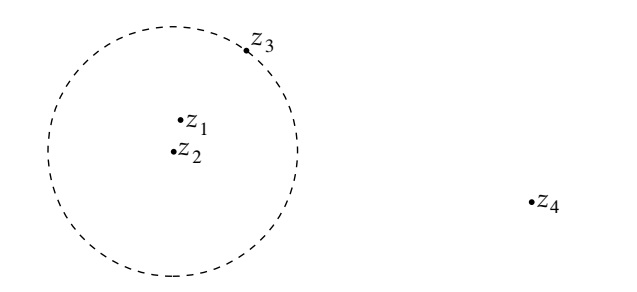
\includegraphics[width=0.6\textwidth]{figure/Fig2.1.jpg}
		\caption{The figure above shows the product of four local operators. The OPE represents the asymptotic behavior as $z_1 \to z_2$ as a series. In this process, a pair of operators at $z_1 , z_2$ is replaced by a single operator at $z_2$.
			The radius of convergence is the distance to other nearest operators, represented by the dashed lines in the figure.    }\label{Fig2.1}
	\end{center}
\end{figure}

The basic objects of study in string perturbation theory are path integral expectation values of products of local operators:    
\begin{equation}
	\left\langle\mathscr{A}_{i_{1}}(z_{1}, \bar{z}_{1}) \mathscr{A}_{i_{2}}(z_{2}, \bar{z}_{2}) \cdots \mathscr{A}_{i_{n}}(z_{n}, \bar{z}_{n})\right\rangle
\end{equation}
where $\mathscr{A}_{i}$ is some basis of the set of local operators. It is very important to understand the behavior of this expectation value in the limit where two of the operators approach each other. A systematic description of this limit is given by the operator product expansion (OPE).    
As shown in Figure \ref{Fig2.1}.    
The OPE states that the product of two local operators close to each other can be approximated to any precision by a sum of local operators:    
\begin{equation}
	\mathscr{A}_{i}(\sigma_{1}) \mathscr{A}_{j}(\sigma_{2})=\sum_{k} c^{k}{}_{i j}(\sigma_{1}-\sigma_{2}) \mathscr{A}_{k}(\sigma_{2}) \:.
	\label{2.2.2}
\end{equation}
This is an operator statement, meaning it holds in a general expectation value:    
\begin{equation}
	\left\langle\mathscr{A}_{i}(\sigma_{1}) \mathscr{A}_{j}(\sigma_{2}) \cdots\right\rangle
	=\sum_{k} c^{k}{}_{i j}(\sigma_{1}-\sigma_{2})\left\langle\mathscr{A}_{k}\left(\sigma_{2}\right) \cdots\right\rangle \label{2.2.3}
\end{equation}
where the distance between $\sigma_{1}, \sigma_{2}$ is smaller than the distance to all other operators. The coefficient function $c^{k}{ }_{i j}(\sigma_{1}-\sigma_{2})$ determines the dependence on the separation, and also depends on $i,j,k$, but is independent of other operators in the expectation value; the dependence on the latter only appears in the expectation value on the right side of (\ref{2.2.3}). These terms are typically arranged in decreasing order of magnitude in the limit $\sigma_{1} \rightarrow \sigma_{2}$.    
Except that the coefficient functions are not simple power series and can be singular as $\sigma_{1} \rightarrow \sigma_{2}$, this is analogous to an ordinary Taylor series.    

We will now use the special properties of free field theory to give a derivation of the OPE for $X^\mu$ theory. In Section 2.9, we will give a derivation for any conformal invariant field theory.    

We have seen that normal products satisfy the equations of motion (\ref{2.1.23}). This indicates that the operator product is a harmonic function of $(z_{1}, \bar{z}_{1})$. A simple result from complex analysis is that a harmonic function is locally the sum of a holomorphic function and an anti-holomorphic function. In particular, it means it is not singular as $z_{1} \rightarrow z_{2}$, and can be freely expanded in a Taylor series in $z_{12}$ and $\bar{z}_{12}$.    
Therefore,    
\begin{align}
	&X^{\mu}(z_{1}, \bar{z}_{1}) X^{v}(z_{2}, \bar{z}_{2})=-\frac{\alpha^{\prime}}{2} \eta^{\mu \nu} \ln \lvert z_{12}\rvert^{2}+ 
	:\mathrel{ X^{v} X^{\mu}(z_{2}, \bar{z}_{2})}:  \nonumber \\
	&\qquad +\sum_{k=1}^{\infty} \frac{1}{k!}\Bigl[(z_{12})^{k}\!
	:\mathrel{X^{v} \partial^{k} X^{\mu}(z_{2}, \bar{z}_{2})}:+
	(\bar{z}_{12})^{k}\!:\mathrel{ X^{v} \bar{\partial}^{k} X^{\mu}(z_{2}, \bar{z}_{2})}:\Bigr] \label{2.2.4}
\end{align}
\begin{tcolorbox}[breakable]
	\begin{remark}
		Here (\ref{2.1.21a}) and    
		\begin{align*}
			&:\mathrel{X^{\mu}(z_{1},\bar{z}_{1}) X^{\nu}(z_{2}, \bar{z}_{2})}:\\
			=&: \mathrel{ X^{\nu} X^{\mu}(z_{2},\bar{z}_{2})}:+\sum_{k=1}^{\infty} \frac{1}{k !}\Bigl[(z_{12})^{k}\!:\mathrel{X^{\nu} \partial^{k} X^{\mu}(z_{2}, \bar{z}_{2})}:+(\bar{z}_{12})^{k}\!:\mathrel{X^{\nu} \bar{\partial}^{k} X^{\mu}(z_{2}, \bar{z}_{2})}:\Bigr]
		\end{align*}
		are used. Because of the equations of motion, the terms with mixed derivatives $\partial \bar{\partial}$ are zero.    
	\end{remark}
\end{tcolorbox}


Equation (\ref{2.2.4}) has the form of an OPE. Like the equation of motion (\ref{2.1.23}) that derived it, this is a statement about operators. For any vacuum expectation value of the product of $X^{\mu}(z_{1},\bar{z}_{1}) X^{v}(z_{2},\bar{z}_{2})$ with fields at other points, its behavior as $z_{1}\to z_{2}$ is an infinite series, where each term is a known function of $z_{12}$ and (or) $\bar{z}_{12}$ multiplied by the expectation value of the local operator that replaces this pair of fields.    

The OPE is usually used as an asymptotic expansion, where the first few terms give the dominant behavior when the separation is very small. Most of our applications will be of this type, and we usually write the OPE as clearly singular terms plus unspecified non-singular remainder terms. Instead of using $=$, we will use "$\sim$" to mean "equal in the sense of differing only by non-singular terms." In fact, the OPE converges in conformal invariant field theories. In certain applications, this is very important to us: it makes it possible to reconstruct the entire theory from the coefficient functions.    
As an example, the radius of convergence of the free field OPE (\ref{2.2.4}) in any given expectation value is equal to the distance from it to the nearest of the other insertions in the path integral, as shown in Figure \ref{Fig2.1}, and the convergence can be proven by standard complex analysis theory.    

Various operators on the right side of the OPE (\ref{2.2.4}) include the product of fields at the same point. In quantum field theory, such products are usually divergent, and thus need to be appropriately truncated and renormalized, but the normal-ordering here makes it well-defined.    
In free field theory, normal-ordering is a convenient way to define composite operators. In interacting field theory, normal-ordering is of little use because composite operators have additional divergences caused by interaction vertices connected to them.    
However, the field theories we are interested in are mostly free field theories, or theories related to free field theories, so more details on normal-ordering are given here.    
Normal-ordering of any number of fields can be defined recursively as    
\begin{align}
	&: \mathrel{ X^{\mu_{1}}(z_{1}, \bar{z}_{1}) \cdots X^{\mu_{n}}(z_{n}, \bar{z}_{n})}: \nonumber \\
	&\qquad\quad =X^{\mu_{1}}(z_{1}, \bar{z}_{1}) \cdots X^{\mu_{n}}(z_{n}, \bar{z}_{n})+\sum \text{subtractions}, \label{2.2.5}
\end{align}
where the subtractions refer to picking one or more pairs of fields from the product of fields and replacing them with $\frac{1}{2} \alpha^{\prime} \eta^{\mu_{i} \mu_{j}} \ln \lvert z_{i j}\rvert^{2}$.    
For example,    
\begin{align}
	&:\mathrel{X^{\mu_{1}}(z_{1}, \bar{z}_{1}) X^{\mu_{2}}(z_{2}, \bar{z}_{2}) X^{\mu_{3}}(z_{3}, \bar{z}_{3})}: = 
	X^{\mu_{1}}(z_{1}, \bar{z}_{1}) X^{\mu_{2}}(z_{2}, \bar{z}_{2}) X^{\mu_{3}}(z_{3}, \bar{z}_{3}) \nonumber \\
	&\qquad+\left(\frac{\alpha^{\prime}}{2} \eta^{\mu_{1} \mu_{2}} \ln \lvert z_{12}\rvert^{2} X^{\mu_{3}}(z_{3}, \bar{z}_{3})+2 \text{ permutations}\right).
	\label{2.2.6}
\end{align}

This definition can be compactly summarized as    
\begin{equation}
	: \mathrel{\mathscr{F}}:=\exp \left(\frac{\alpha^{\prime}}{4} \int \dif^{2} z_{1} \dif^{2} z_{2} \ln \lvert z_{12}\rvert^{2}\: 
	\frac{\delta}{\delta X^{\mu}(z_{1}, \bar{z}_{1})} \frac{\delta}{\delta X_{\mu}(z_{2}, \bar{z}_{2})}\right) \mathscr{F} \:, \label{2.2.7}
\end{equation}
where $\mathscr{F}$ is any functional of $X$.    
This is equivalent to equation (\ref{2.2.5}): the double functional derivative in the exponent contracts each pair of fields, and summing the exponent of multiple pairings cancels out the fractions in the derivative action. An application of this formal expression is to apply the inverse of the exponent on both sides, which gives    
\begin{align}
	\mathscr{F} &=\exp \left(-\frac{\alpha^{\prime}}{4} \int \dif^{2} z_{1} \dif^{2} z_{2} \ln \lvert z_{12}\rvert^{2}\: 
	\frac{\delta}{\delta X^{\mu}(z_{1}, \bar{z}_{1})} \frac{\delta}{\delta X_{\mu}(z_{2}, \bar{z}_{2})}\right):\mathrel{\mathscr{F}}: \nonumber \\
	&=: \mathrel{\mathscr{F}}:+\sum \text {contractions}\:, \label{2.2.8}
\end{align}
where the contractions are the inverse of subtractions: picking one or more pairs of fields from $:\mathrel{\mathscr{F}}:$ and replacing them with $-\frac{1}{2} \alpha^{\prime} \eta^{\mu_{i} \mu_{j}} \ln \lvert z_{i j}\rvert^{2}$.    
For any functionals $\mathscr{F}$ and $\mathscr{G}$ of $X$, their OPE is generated by    
\begin{equation}
	: \mathrel{\mathscr{F}}: :\mathrel{\mathscr{G}}:=: \mathrel{\mathscr{F} \mathscr{G}}:+\sum \text{cross contractions}
\end{equation}
The cross contractions now refer to contracting a field in $\mathscr{F}$ and a field in $\mathscr{G}$ and summing over them. This can also be written as    
\begin{equation}
	: \mathrel{\mathscr{F}}: :\mathrel{\mathscr{G}}:= \exp \left(-\frac{\alpha^{\prime}}{2} 
	\int \dif^{2} z_{1} \dif^{2} z_{2}\: \ln \lvert z_{12}\rvert^{2} \frac{\delta}{\delta X_{F}^{\mu}(z_{1}, \bar{z}_{1})} 
	\frac{\delta}{\delta X_{G \mu}(z_{2}, \bar{z}_{2})}\right): \mathrel{\mathscr{F} \mathscr{G}}: \label{2.2.10}
\end{equation}
where the functional derivatives only act on fields in $\mathscr{F}$ or $\mathscr{G}$ respectively.    
As an example,    
\begin{align}
	&: \mathrel{\partial X^{\mu}(z) \partial X_{\mu}(z)}: : \mathrel{\partial^{\prime} X^{v}(z^{\prime}) \partial^{\prime} X_{v}(z^{\prime})}: \nonumber \\
	&\qquad \qquad \qquad =: \mathrel{\partial X^{\mu}(z) \partial X_{\mu}(z) \partial^{\prime} X^{v}(z^{\prime}) \partial^{\prime} X_{v}(z^{\prime})}: \nonumber\\
	&\qquad \qquad \qquad \qquad \qquad {-}4 \cdot \frac{\alpha^{\prime}}{2}
	(\partial \partial^{\prime} \ln \lvert z-z^{\prime}\rvert^{2}): \mathrel{\partial X^{\mu}(z) \partial^{\prime} X_{\mu}(z^{\prime})}: \nonumber\\
	&\qquad \qquad \qquad \qquad \qquad {+}2 \cdot \eta^{\mu}{ }_{\mu}\left(-\frac{\alpha^{\prime}}{2} \partial \partial^{\prime}
	\ln \lvert z-z^{\prime}\rvert^{2}\right)^{2} \nonumber\\
	&\qquad \qquad \qquad \sim \frac{D \alpha^{\prime 2}}{2(z-z^{\prime})^{4}}-\frac{2 \alpha^{\prime}}{(z-z^{\prime})^{2}}
	: \mathrel{\partial^{\prime} X^{\mu}(z^{\prime}) \partial^{\prime} X_{\mu}(z^{\prime})}: \nonumber\\
	&\qquad \qquad \qquad \qquad \qquad {-}\frac{2 \alpha^{\prime}}{z-z^{\prime}}: \mathrel{\partial^{\prime 2} X^{\mu}\left(z^{\prime}\right) \partial^{\prime} X_{\mu}\left(z^{\prime}\right)}:\:.
	\label{2.2.11}
\end{align}
The second term after the equal sign comes from the four ways to contract a single pair of fields, while the third term comes from the two ways to contract two pairs of fields. In the last line, we write the OPE in standard form by performing a Taylor expansion inside the normal ordering: each operator in each term is at $z'$, and arranged in order of singularity.    

\begin{tcolorbox}[breakable]
	\begin{remark}
		The second term after the equal sign comes from    
		\begin{align*}
			\wick{ : \partial \c1 {X}^{\mu}(z) \partial X_{\mu}(z) : : \partial^{\prime} \c1 {X}^{\nu} (z^{\prime}) \partial^{\prime} X_{\nu}(z^{\prime}) : }
			&=\partial \partial^{\prime}\left(-\frac{\alpha^{\prime}}{2} \eta^{\mu \nu}\ln \lvert z-z^{\prime}\rvert^{2}\right) 
			: \mathrel{\partial X_{\mu}(z) \partial X_{\nu}(z)}: \\
			&=-\frac{\alpha^{\prime}}{2} \Bigl(\partial \partial^{\prime} \ln \lvert z-z^{\prime}\rvert^{2}\Bigr)  
			: \mathrel{\partial X_{\mu}(z) \partial^{\prime} X^{\mu}(z)}:
		\end{align*}
		while the third term comes from
		\begin{align*}
		\wick{ : \partial \c1 {X}^{\mu}(z) \partial \c2 {X}_{\mu}(z) : : \partial^{\prime} \c1 {X}^{\nu}(z^{\prime}) \partial^{\prime} \c2 {X}_{\nu}(z^{\prime}) : } 
			&=\partial \partial^{\prime}\left(-\frac{\alpha^{\prime}}{2} \eta ^{\mu \nu} \ln \lvert z-z^{\prime}\rvert^{2}\right) 
			\partial \partial^{\prime}\left(-\frac{\alpha^{\prime}}{2} \eta_{\mu \nu}\ln \lvert z-z^{\prime}\rvert^{2}\right) \\
			&=\eta^{\mu \nu} \eta_{\mu \nu}\left(-\frac{\alpha^{\prime}}{2} \partial \partial^{\prime}\ln \lvert z- z^{\prime}\rvert ^{2}\right)^{2}
		\end{align*}
		Because $\eta^{\mu \nu} \eta_{\nu\rho}=\delta^{\mu}{}_{\rho}$, so $\eta^{\mu \nu} \eta_{\mu \nu}=\delta^{\mu}{ }_{\mu}=D$, and then using    
		$
		\partial \partial^{\prime} \ln \lvert z-z^{\prime }\vert 
		^{2}= (z-z^{\prime})^{-2}
		$
		and    
		\[
		:\mathrel{\partial X^\mu(z)\partial^\prime X_{\mu}(z^\prime)}:\sim :\mathrel{\partial^\prime X^\mu(z^\prime)\partial^\prime X_\mu(z^\prime)}: 
		+ \:(z-z^\prime):\mathrel{\partial^{\prime 2} X^\mu(z^\prime)\partial^\prime X_\mu(z)}:
		\]
		(\ref{2.2.11}) is obtained.    
	\end{remark}
\end{tcolorbox}


Another important example is    
\begin{equation}
	\mathscr{F}=\me^{\mi k_{1} \cdot X(z, \bar{z})}, \qquad \mathscr{G}=\me^{\mi k_{2} \cdot X(0,0)}
\end{equation}
The variations $\delta / \delta X_{F}^{\mu}$ and $\delta / \delta X_{G}^{\mu}$ yield the factors $\mi k_{1 \mu}$ and $\mi k_{2 \mu}$ respectively, so the general result (\ref{2.2.10}) becomes    
\begin{align}
	:\mathrel{\me^{\mi k_{1} \cdot X(z, \bar{z})}}: : \mathrel{\me^{\mi k_{2} \cdot X(0,0)}}: 
	&=\exp \left(\frac{\alpha^{\prime}}{2} k_{1} \cdot k_{2} \ln |z|^{2}\right) :\mathrel{\me^{\mi k_{1} \cdot X(z, \bar{z})} \me^{\mi k_{2} \cdot X(0,0)}} : \nonumber \\
	&=|z|^{\alpha^{\prime} k_{1} \cdot k_{2}}: \mathrel{ \me^{\mi k_{1} \cdot X(z, \bar{z})} \me^{\mi k_{2} \cdot X(0,0)}}: \:.
	\label{2.2.13}
\end{align}
To derive the OPE, Taylor expansion in the normal ordering gives    
\begin{equation}
	:\mathrel{\me^{\mi k_{1} \cdot X(z, \bar{z})}}: : \mathrel{\me^{\mi k_{2} \cdot X(0,0)}}: 
	=|z|^{\alpha^{\prime} k_{1} \cdot k_{2}}: \mathrel{\me^{\mi(k_{1}+k_{2}) \cdot X(0,0)}[1+O(z, \bar{z})]}: \:.\label{2.2.14}
\end{equation}
\begin{tcolorbox}[breakable]
	\begin{remark}
		The general result (\ref{2.2.10}) here is    
		\begin{align*}
			&:\mathrel{ \me^{i k_{1} \cdot X(z,\bar{z})}}::\mathrel{\me^{\mi k_{2} \cdot X(0,0)}}:\\
			&\quad =\left(1-\frac{\alpha^{\prime}}{2} \int \dif^{2} z_{1} \dif^{2} z_{2}\: \ln \lvert z_{12}\rvert^{2} \frac{\delta}{\delta X_{F}^{\mu}(z_{1},\bar{z}_{1})} \frac{\delta}{\delta X_{G \mu}(z_{2}, \bar{z}_{2})} +\cdots \right):\mathrel{ \me^{\mi k_{1} \cdot X(z, \bar{z})} \me^{\mi k_{2} \cdot X(0,0)}}:\\
			&\quad =:\mathrel{\me^{\mi k_{1} \cdot X(z, \bar{z})} \me^{\mi k_{2} \cdot X(0,0)}}: \\ 
			&\quad \quad \times \left(1 -\frac{\alpha^{\prime}}{2} \int \dif^{2} z_{1} \dif^{2} z_{2}\: \ln \lvert z_{12}\rvert ^{2}
			\times \mi k_{1 \mu} \delta^{2}(z-z_{1}, \bar{z}-\bar{z}_{1}) \mi k_{2}^{\mu} \delta^{2}(0-z_{2}, 0,-\bar{z}_{2})+ \cdots \right)\\
			&\quad =:\mathrel{\me^{\mi k_{1} \cdot X(z, \bar{z})} \me^{\mi k_{2} \cdot X(0,0)}}: 
			\left(1+\frac{\alpha^{\prime}}{2} k_{1} \cdot k_{2} \ln |z|^{2}+\cdots\right)=
			|z|^{\alpha^{\prime} k_{1} \cdot k_{2}}: \mathrel{ \me^{\mi k_{1} \cdot X(z, \bar{z})} \me^{\mi k_{2} \cdot X(0,0)}}: \:.
		\end{align*}
	\end{remark}
\end{tcolorbox}

Note that OPEs such as (\ref{2.2.2}), (\ref{2.2.4}) are non-symmetric with respect to $\sigma_{1}$ and $\sigma_{2}$. These OPEs can be reshaped into a symmetric form by expanding around $(\sigma_{1}+\sigma_{2})/ 2$.    
The coefficient functions in the symmetric form satisfy, under the exchange of two operators:    
\begin{equation}
	c^{k}{}_{ij}(\sigma_{1}-\sigma_{2})_{\mathrm{sym}}= \pm c^{k}{}_{j i}(\sigma_{2}-\sigma_{1})_{\mathrm{sym}} \:,
\end{equation}
where the sign is negative when $\mathscr{A}_{i}$ and $\mathscr{A}_{j}$ are both anti-commuting.    


\section{\texorpdfstring{Ward identities and Noether theorem}{2.3 Ward identities and Noether theorem}}

Worldsheet symmetry plays an important role in string theory.    
In this section, we first derive some general results for symmetry in field theory.    

Consider a field theory in $d$-dimensional spacetime with action $S_\phi$, where $\phi_\alpha(\sigma)$ labels a general field. Suppose it has the symmetry    
\begin{equation} \label{2.3.1}
	\phi_{\alpha}^{\prime}(\sigma)=\phi_{\alpha}(\sigma)+\delta \phi_{\alpha}(\sigma) \:,
\end{equation}
where $\delta \phi_\alpha$ is proportional to an infinitesimal parameter $\epsilon$. The product of the path integral measure and the weight $\exp(-S)$ is invariant:    
\begin{equation} \label{2.3.2}
	[\dif \phi^{\prime}]\: \exp(-S[\phi^{\prime}])=[\dif  \phi] \exp (-S[\phi]) \:.
\end{equation}

In field theory, a continuous symmetry implies the existence of a conserved current (Noether's theorem) and Ward identities (which constrain operator products of the current). To derive these results, consider the field variation    
\begin{equation}\label{2.3.3}
	\phi_{\alpha}^{\prime}(\sigma)=\phi_{\alpha}(\sigma)+\rho(\sigma) \delta \phi_{\alpha}(\sigma)
\end{equation}
This is not a symmetry, but $[\dif \phi]\exp(-S)$ is invariant when $\rho$ is a constant, so its variation must be proportional to $\partial _a \rho$:    
\begin{align}
	&[\dif \phi^{\prime}]\: \exp (-S[\phi^{\prime}]) \nonumber \\
	&\qquad=[\dif \phi] \: \exp (-S[\phi])\left[1+\frac{\mi \epsilon}{2 \pi} \int \dif^{d} \sigma\: 
	g^{1 / 2} j^{a}(\sigma) \partial_{a} \rho(\sigma)+O\left(\epsilon^{2}\right)\right] \label{2.3.4}
\end{align}
The unknown coefficient $j^a(\sigma)$ comes from the variation of the measure and the action.    
Take $\rho$ to be non-zero only in a small region. Outside this region, consider a path integral containing a general insertion "$\cdots$".    
This insertion is invariant under (\ref{2.3.3}):    
\begin{align}
	0 &=\int[\dif \phi^{\prime}]\: \exp (-S[\phi^{\prime}]) \cdots \: - \: \int[\dif \phi] \exp (-S[\phi]) \cdots \nonumber \\
	&=\frac{\mi \epsilon}{2 \pi} \int \dif^{d} \sigma\: 
	g^{1 / 2} j^{a}(\sigma) \partial_{a} \rho(\sigma)+O(\epsilon^2)=\frac{\epsilon}{2 \pi \mi} \int \dif^{d} \sigma \: g^{1 / 2} \rho(\sigma)\left\langle\nabla_{a} j^{a}(\sigma) \cdots\right\rangle
	\label{2.3.5}
\end{align}
thus we have    
\begin{equation}
	\nabla_{a} j^{a}=0 \:.
	\label{2.3.6}
\end{equation}
\begin{tcolorbox}[breakable]
	\begin{proof}
		We use the fact that \( \partial_a (g^{1/2} v^a(c)) = g^{1/2} \nabla_a v^a(c) \) as shown here
		
		\[
		\begin{aligned}
			\text{LHS} = \partial_a (\sqrt{g} v^a) &= (\partial_a \sqrt{g}) v^a + \sqrt{g} \partial_a v^a \\
			&= \frac{1}{2\sqrt{g}} g g^{bc} \partial_a g_{bc} v^a + \sqrt{g} \partial_a v^a \\
			&= \sqrt{g} \left( \frac{1}{2} g^{bc} \partial_a g_{bc} v^a + \partial_a v^a \right)
		\end{aligned}
		\]
		
		For the RHS we find
		
		\[
		\begin{aligned}
			\text{RHS} = \sqrt{g} \nabla_a v^a &= \sqrt{g} \left( \partial_a v^a + \Gamma^a_{ab} v^b \right) \\
			&= \sqrt{g} \left[ \partial_a v^a + \frac{1}{2} (g^{ac} \partial_a g_{cb} + g^{ac} \partial_b g_{ca} - g^{ac} \partial_c g_{ab}) v^b \right] \\
			&= \sqrt{g} \left( \partial_a v^a + \frac{1}{2} g^{ac} \partial_b g_{ca} v^b \right)
		\end{aligned}
		\]
		
		The second and last term of the connection cancel after interchanging the dummy indices \( a \) and \( c \). This is now equal to the LHS.
		
		To derive \eqref{2.3.5} we start from \eqref{2.3.4}, which implies
		
		\[
		\begin{aligned}
			0 &= \frac{\mi \epsilon}{2 \pi}\int d^d \sigma \, g^{1/2} j^a(\sigma) \partial_a \rho(\sigma) \\
			&= -\frac{\mi \epsilon}{2 \pi}\int d^d \sigma \, \partial_a (g^{1/2} j^a(\sigma)) \rho(\sigma) \\
			&= \frac{\epsilon}{2 \pi i}\int d^d \sigma \, g^{1/2} \nabla_a j^a(\sigma) \rho(\sigma)
		\end{aligned}
		\] 
	\end{proof}    
\end{tcolorbox}

To derive Ward identities, let $\rho(\sigma)$ be 1 in region $R$ and 0 outside $R$. Additionally, introduce a general local operator $\mathscr{A}(\sigma_{0})$ at a point $\sigma_{0}$ within the path integral region $R$.    
Inserting arbitrary operators "$\cdots$" outside $R$ gives    
\begin{equation} \label{2.3.7}
	\delta \mathscr{A}(\sigma_{0})+\frac{\epsilon}{2 \pi \mi} \int_{R} \dif^{d} \sigma \: g^{1 / 2} \nabla_{a} j^{a}(\sigma) \mathscr{A}(\sigma_{0})=0 \:.
\end{equation}

\begin{tcolorbox}[breakable]
	\begin{proof}
		Similar to (\ref{2.3.5}), using $\partial_a\rho\big\lvert_{|z|=R}\ne0$ we now have    
		\[
		0=\int [\dif \phi]\:\me^{-S[\phi]}\biggl(\delta\mathscr{A}(\sigma_{0})+\frac{\mi\epsilon}{2\pi}\int \dif^{d}\sigma \: 
		j^{a}(\sigma)\partial_{a}\rho(\sigma)\mathscr{A}(\sigma_{0}) \biggr) \cdots     \:,
		\]
		then using integration by parts, (\ref{2.3.7}) can be obtained.    
	\end{proof}
\end{tcolorbox}
\noindent Equivalently,    
\begin{equation}
	\nabla_{a} j^{a}(\sigma) \mathscr{A}(\sigma_{0})=g^{-1 / 2} \delta^{d}(\sigma-\sigma_{0}) \frac{2 \pi}{\mi \epsilon} \delta \mathscr{A}(\sigma_{0})+\sigma \:\text{total derivative} \:.
	\label{2.3.8}
\end{equation}
Divergence theorem gives    
\begin{equation}
	\int_{\partial R} \dif A\: n_{a} j^{a} \mathscr{A}(\sigma_{0})=\frac{2 \pi}{\mi \epsilon} \delta \mathscr{A}(\sigma_{0}) \:,\label{2.3.9}
\end{equation}
where $\dif A$ is the area element, and $n_{a}$ is the outward normal vector.    
In 2-dimensional flat space, this is    
\begin{equation} \label{2.3.10}
	\oint_{\partial R}(j\dif z-\tilde{\jmath} \dif \bar{z}) \mathscr{A}(z_{0}, \bar{z}_{0})
	=\frac{2 \pi}{\epsilon} \delta \mathscr{A}(z_{0}, \bar{z}_{0})
\end{equation}
Here we have dropped the indices $j \equiv j_{z}$, $\tilde{\jmath} \equiv j_{\bar{z}}$. We use $\tilde{\jmath}$ instead of $\bar{\jmath}$ because $\tilde{\jmath}$ is not the conjugate of $j$.    
The Minkowski density $j_0$ is generally Hermitian, $(j_{z})^{\dagger}=\frac{1}{2}(j_{1}-\mi j_{2})^{\dagger}=j_{z}$.    
\begin{tcolorbox}[breakable]
	\begin{proof}
		The proof of (\ref{2.3.9}) used    
		\[
		\int_{R} \dif^{d} \sigma \: g^{1 / 2} \nabla_{a} j^{a} =\int_{R} \dif ^d \sigma \: \partial_{a}\bigl(g^{1 / 2} j^{a}\bigr) 
		=\int_{\partial R} \dif A\: n_{\alpha} j^{a} \:,
		\]
		Using the two-dimensional Stokes' theorem     $
		\int_{R} \dif^{2}z\: \bigl(\partial_{z} v^{z}+\partial_{\bar{z} } v^{\bar{z}}\bigr)=\mi \oint_{\partial R}(v^{z} \dif \bar{z}-v^{\bar{z}} \dif \bar{z})
		$ (\ref{2.3.10}) is obtained.    
	\end{proof}
\end{tcolorbox}

Importantly, the Noether theorem and Ward identities are local properties, and do not depend on distant boundary conditions, nor on whether they are invariant under the symmetry. In particular, because $\rho(\sigma)$ is only non-zero in $R$, only symmetry transformations in $R$ need to be defined.    

In conformal invariant theories, usually $j_z$ is holomorphic and $j_{\bar{z}}$ is anti-holomorphic. In this case, the currents $(j_z,0)$ and $(0,j_{\bar{z}})$ are separately conserved.    
Thus the integral yields the residue in the OPE:    
\begin{equation}\label{2.3.11}
	\operatorname{Res}_{z \to z_{0}} j(z) \mathscr{A}(z_{0}, \bar{z}_{0})+\overline{\operatorname{Res}}_{\bar{z} \to \bar{z}_{0}} \, \tilde{\jmath}(\bar{z}) \mathscr{A}(z_{0}, \bar{z}_{0})=\frac{1}{\mi \epsilon} \delta \mathscr{A}(z_{0}, \bar{z}_{0})
\end{equation}
Here $\operatorname{Res},\overline{\operatorname{Res}}$ refer to taking the coefficients of $(z-z_{0})^{-1}$ and $(\bar{z}-\bar{z}_{0})^{-1}$ respectively.    

An example: Returning to the massless free scalar field, and consider \emph{spacetime} translations $\delta X^{\mu}=\epsilon a^{\mu}$.    
Under $\delta X^{\mu}(\sigma)=\epsilon \rho(\sigma) a^{\mu}$,    
\begin{align}
	\delta S=\frac{1}{4 \pi \alpha^{\prime}} \int \dif^{2}\sigma\: 2(\delta \partial^{a} X^{\mu}) \partial_{a} X_{\mu} 
	=\frac{\epsilon a_{\mu}}{2 \pi \alpha^{\prime}} \int \dif^{2} \sigma \:\partial^{a} X^{\mu} \partial_{a} \rho \:.
\end{align}
This is equivalent to taking the Noether current in (\ref{2.3.5}) as $j_{a}(\sigma)=a_{\mu} j_{a}^{\mu}$, where    
\begin{equation}
	j_{a}^{\mu}=\frac{\mi}{\alpha^{\prime}} \partial_{a} X^{\mu} \:. \label{2.3.13}
\end{equation}
The OPE of the current and the exponential operator gives    
\begin{subequations} \label{2.3.14}
	\begin{align}
		j^{\mu}(z): \mathrel{\me^{\mi k \cdot X(0,0)}}: &\sim \frac{k^{\mu}}{2 z}: \mathrel{\me^{\mi k \cdot X(0,0)}}:  \:,\label{2.3.14a} \\
		\tilde{\jmath}^{\mu}(\bar{z}):\mathrel{ \me^{\mi k \cdot X(0,0)}}: &\sim \frac{k^{\mu}}{2 \bar{z}}: 
		\mathrel{\me^{\mi k \cdot X(0,0)}}:\:.
		\label{2.3.14b}
	\end{align}
\end{subequations}
\begin{tcolorbox}[breakable]
	\begin{proof}
		Explanation for (\ref{2.3.14a}): from (\ref{2.3.13}) it can be obtained that $j^{\mu}=j_{z}^{\mu}=\frac{\mi}{\alpha^{\prime}} \partial_{z} X^{\mu}$, so    
	\begin{align}
		 \frac{i}{\alpha'} \partial X^\mu(z)
		: \sum_{n=0}^{\infty} \frac{i^n}{n!} (k \cdot X(0))^n : &= \frac{i}{\alpha'} 
		: \sum_{n=0}^{\infty} \frac{i^n}{n!} 
		\, \partial X^\mu(z) (k \cdot X(0))^n : \notag\\[6pt]
		&\sim \frac{i}{\alpha'} 
		: \sum_{n=1}^{\infty} \frac{i^n}{n!} 
		\sum_{i=1}^{n}
		\wick{ \c{\partial X^\mu(z)} (k \cdot \c{X(0)}) }_{i}
		\prod_{j\ne i}(k \cdot X(0))_j : \notag\\[6pt]
		&= \frac{i}{\alpha'} 
		: \sum_{n=1}^{\infty} \frac{i^n}{n!} 
		\, n \, \wick{ \c{\partial X^\mu(z)} (k \cdot \c{X(0)}) }
		(k \cdot X(0))^{n-1} : \notag\\[6pt]
		&= \frac{i}{\alpha'} \left(-\frac{\alpha'}{2}\eta^{\mu\nu}\partial\ln(z\bar{z})\right)k_{\nu} 
		: \sum_{n=1}^{\infty} \frac{i^n}{(n-1)!} 
		(k \cdot X(0))^{n-1} : \notag\\[6pt]
		&= \frac{i}{\alpha'} 
		\left(-\frac{\alpha'}{2} \frac{k^\mu}{z} \right)
		: \sum_{n=1}^{\infty} \frac{i^n}{(n-1)!} (k \cdot X(0))^{n-1} : \notag\\[6pt]
		&= \frac{k^\mu}{2z} : e^{ik \cdot X(0)} :.\label{ope: derivX-exp}
	\end{align}
	Alternatively, we can use
	\begin{equation}
		:F::G:
		=
		\exp\!\left(
		-\frac{\alpha'}{2}
		\int d^2 z_1 d^2 z_2 \,
		\log |z_{12}|^2\,
		\frac{\delta}{\delta X_F^\mu(z_1,\bar z_1)}
		\frac{\delta}{\delta X_{G\mu}(z_2,\bar z_2)}
		\right)
		:FG: .
	\end{equation}
	
	This gives
	\begin{align}
		:\frac{i}{\alpha'}\partial X^\mu(z)::e^{ik\cdot X(w,\bar w)}:
		&=
		\exp\!\left(
		-\frac{\alpha'}{2}
		\int d^2 z_1 d^2 z_2\,
		\log |z_{12}|^2\,
		\frac{\delta}{\delta X_F^\mu(z_1,\bar z_1)}
		\frac{\delta}{\delta X_{G\mu}(z_2,\bar z_2)}
		\right)\notag\\
		&\qquad\times:\frac{i}{\alpha'}\partial X^\mu(z)e^{ik\cdot X(w,\bar w)}:
		\\[1ex]
		&=
		:\frac{i}{\alpha'}\partial X^\mu(z)e^{ik\cdot X(w,\bar w)}:
		\nonumber\\
		&\quad
		-\frac{i}{2}
		:
		\int d^2 z_1 d^2 z_2\,
		\log |z_{12}|^2
		\frac{\delta(\partial X^\mu(z))}{\delta X_F^\mu(z_1,\bar z_1)}
		\frac{\delta(e^{ik\cdot X(w,\bar w)})}{\delta X_{G\mu}(z_2,\bar z_2)}
		:
		\nonumber\\[1ex]
		&=
		:\frac{i}{\alpha'}\partial X^\mu(z)e^{ik\cdot X(w,\bar w)}:
		\nonumber\\
		&\quad
		+\frac{i}{2}
		:
		\int d^2 z_1 d^2 z_2\,
		\log |z_{12}|^2\,
		\partial\!\left(
		\delta^\mu_{\ \alpha}\delta^2(z_1,z)
		\right)
		ik^\alpha \delta^2(z_2,w)
		e^{ik\cdot X(w,\bar w)}
		:
		\nonumber\\[1ex]
		&=
		:\frac{i}{\alpha'}\partial X^\mu(z)e^{ik\cdot X(w,\bar w)}:
		\nonumber\\
		&\quad
		+\frac{k^\mu}{2}
		:
		\partial\!\left(
		\int d^2 z_1 d^2 z_2\,
		\log |z_{12}|^2
		\delta^2(z_1,z)\delta^2(z_2,w)
		e^{ik\cdot X(w,\bar w)}
		\right)
		:
		\nonumber\\[1ex]
		&=
		:\frac{i}{\alpha'}\partial X^\mu(z)e^{ik\cdot X(w,\bar w)}:
		+
		\frac{k^\mu}{2}
		:
		\partial\!\left(
		\log |z-w|^2
		e^{ik\cdot X(w,\bar w)}
		\right)
		:
		\nonumber\\[1ex]
		&=
		:\frac{i}{\alpha'}\partial X^\mu(z)e^{ik\cdot X(w,\bar w)}:
		+
		\frac{k^\mu}{2(z-w)}
		:
		e^{ik\cdot X(w,\bar w)}
		: .
	\end{align}
	where we used the fact that $z_1\ne z_2$ to drop higher order terms. Therefore
	\begin{equation}
		:j^\mu(z)::e^{ik\cdot X(w,\bar w)}:
		\sim
		\frac{k^\mu}{2(z-w)}
		:e^{ik\cdot X(w,\bar w)}: .
	\end{equation}
	QED.
	\end{proof}
\end{tcolorbox}

Another example: worldsheet translations $\delta \sigma^{a}=\epsilon v^{a}$, then $\delta X^{\mu}=-\epsilon v^{a} \partial_{a} X^{\mu}$, the Noether current is    
\begin{subequations}
	\begin{align}
		j_{a}  &=\mi v^{b} T_{a b} \:, \label{2.3.15a} \\
		T_{a b}&=-\frac{1}{\alpha^{\prime}}:\mathrel{\biggl(\partial_{a} X^{\mu} \partial_{b} X_{\mu}-\frac{1}{2} \delta_{a b} \partial_{c} X^{\mu} \partial^{c} X_{\mu}\biggr)}: \:.
		\label{2.3.15b}
	\end{align}
\end{subequations}

 \begin{tcolorbox}[breakable]
\begin{proof}
	Consider a local worldsheet translation $\delta \sigma^{a} = \epsilon^{a}(\sigma)$. The corresponding variation of the scalar field is:
	$$ \delta X^{\mu} = -\epsilon^{a}(\sigma) \partial_{a} X^{\mu} $$
	The variation of the Polyakov action (in conformal gauge) is given by:
	\begin{align*}
		\delta S &= \frac{1}{4\pi \alpha'} \int d^{2} \sigma \, 2\partial_{b} (\delta X^{\mu}) \partial^{b} X_{\mu} \\
		&= -\frac{1}{2\pi \alpha'} \int d^{2} \sigma \, \partial_{b} (\epsilon^{a} \partial_{a} X^{\mu}) \partial^{b} X_{\mu} \\
		&= -\frac{1}{2\pi \alpha'} \int d^{2} \sigma \left[ (\partial_{b} \epsilon^{a}) \partial_{a} X^{\mu} \partial^{b} X_{\mu} + \epsilon^{a} (\partial_{b} \partial_{a} X^{\mu} \partial^{b} X_{\mu}) \right]
	\end{align*}
	Using the identity $\partial_{a} (\partial_{c} X^{\mu} \partial^{c} X_{\mu}) = 2 \partial_{b} \partial_{a} X^{\mu} \partial^{b} X_{\mu}$, we rewrite the second term:
	$$ \delta S = -\frac{1}{2\pi \alpha'} \int d^{2} \sigma \left[ (\partial_{b} \epsilon^{a}) \partial_{a} X^{\mu} \partial^{b} X_{\mu} + \frac{1}{2} \epsilon^{a} \partial_{a} (\partial_{c} X^{\mu} \partial^{c} X_{\mu}) \right] $$
	Performing integration by parts on the second term (and assuming $\epsilon^a$ vanishes at infinity):
	$$ \int d^{2} \sigma \, \epsilon^{a} \partial_{a} (\partial_{c} X^{\mu} \partial^{c} X_{\mu}) = - \int d^{2} \sigma (\partial_{a} \epsilon^{a}) (\partial_{c} X^{\mu} \partial^{c} X_{\mu}) $$
	Substituting $\partial_{a} \epsilon^{a} = \delta^{b}_{a} \partial_{b} \epsilon^{a}$ allows us to factor out the derivative of the parameter:
	\begin{align*}
		\delta S &= -\frac{1}{2\pi \alpha'} \int d^{2} \sigma \left[ (\partial_{b} \epsilon^{a}) \partial_{a} X^{\mu} \partial^{b} X_{\mu} - \frac{1}{2} (\partial_{b} \epsilon^{a}) \delta^{b}_{a} (\partial_{c} X^{\mu} \partial^{c} X_{\mu}) \right] \\
		&= \frac{1}{2\pi} \int d^{2} \sigma (\partial_{b} \epsilon^{a}) \left[ -\frac{1}{\alpha'} \left( \partial_{a} X^{\mu} \partial^{b} X_{\mu} - \frac{1}{2} \delta^{b}_{a} \partial_{c} X^{\mu} \partial^{c} X_{\mu} \right) \right]
	\end{align*}
	By the definition of the Noether current $\delta S = \frac{1}{2\pi} \int d^2\sigma (\partial^b \epsilon^a) j_{ab}$, we identify:
	$$ T_{ab} = -\frac{1}{\alpha'} \left( \partial_{a} X^{\mu} \partial_{b} X_{\mu} - \frac{1}{2} \delta_{ab} \partial_{c} X^{\mu} \partial^{c} X_{\mu} \right) $$
	The current for a translation $v^a$ is then $j_a = iv^b T_{ab}$.
\end{proof}
 \end{tcolorbox}


\section{\texorpdfstring{Conformal invariance}{2.4 Conformal invariance}}

The energy-momentum tensor (\ref{2.3.15b}) is traceless: $T_a{}^a=0$.    
In complex coordinates using \eqref{matrix-metric}, we have: 
\begin{equation}
	g^{ab}T_{ab}=\underbrace{g^{zz}}_{=0}T_{zz}+2g^{z\bar{z}}T_{z\bar{z}}+\underbrace{g^{\bar{z}\bar{z}}}_{=0}T_{\bar{z}\bar{z}}\implies T_{z \bar{z}}=0\:. \label{2.4.1}
\end{equation}
The conservation law $\partial^a T_{ab}=0$ implies that in any theory with $T_a{}^a=0$    
\begin{equation}
	\bar{\partial} T_{z z}=\partial T_{\bar{z} \bar{z}}=0 \:. \label{2.4.2}
\end{equation}
Therefore    
\begin{equation}
	T(z) \equiv T_{z z}(z)\:, \qquad \tilde{T}(\bar{z}) \equiv T_{\bar{z} \bar{z}}(\bar{z}) \label{2.4.3}
\end{equation}
are holomorphic and anti-holomorphic respectively.    
For massless free scalars    
\begin{equation}\label{2.4.4}
	T(z)=-\frac{1}{\alpha^{\prime}}: \mathrel{\partial X^{\mu} \partial X_{\mu}}: \:, \qquad 
	\tilde{T}(\bar{z})=-\frac{1}{\alpha^{\prime}}:\mathrel{ \bar{\partial} X^{\mu} \bar{\partial} X_{\mu}}: \:,
\end{equation}
according to the equations of motion, they are indeed holomorphic and anti-holomorphic.    


The tracelessness of $T_{ab}$ implies a much larger symmetry.    
The currents    
\begin{equation}
	j(z)=\mi v(z) T(z) \:, \qquad \tilde{\jmath}(\bar{z})=\mi v(z)^{*} \tilde{T}(\bar{z}) \label{2.4.5}
\end{equation}
are conserved for holomorphic $v(z)$.    
\begin{tcolorbox}[breakable]
	\begin{proof}
		\text{Denote } $j_{z}=i v^{z} T_{z z}$, $j_{\bar{z}}=i v^{\bar{z}} T_{\bar{z} \bar{z}}$.    
		\text{So } $
		\nabla_{a} j^{a}= \bar{\partial} j_{z}+\partial j_{\bar{z}}=0$.    
	\end{proof}    
\end{tcolorbox}
For free scalar theory, the OPE is obtained    
\begin{equation} \label{2.4.6}
	T(z) X^{\mu}(0) \sim \frac{1}{z} \partial X^{\mu}(0), \quad \tilde{T}(\bar{z}) X^{\mu}(0) \sim \frac{1}{\bar{z}} \bar{\partial} X^{\mu}(0)
\end{equation}
% \begin{proof}
	% $$
	% T(z)=-\frac{1}{\alpha^{\prime}}: \partial X^{\mu} \partial X_{\mu}:
	% $$
	% $$
	% -\frac{1}{\alpha^{\prime}}: \partial X^{\mu} \partial X_{\mu}: X^{\nu}(0)=-\frac{1}{\alpha^{\prime}}: \partial X^{\mu} \partial X_{\mu}(z) X^{\nu}(0):\sim \frac{1}{z} \partial X_{\mu} (0)
	% $$
	% \end{proof}
then the Ward identity gives the transformation    
\begin{equation}\label{2.4.7}
	\delta X^{\mu}=-\epsilon v(z) \partial X^{\mu}-\epsilon v(z)^{*} \bar{\partial} X^{\mu}
\end{equation}
This is the infinitesimal coordinate transformation $z^{\prime}=z+\epsilon v(z)$.    
The finite transformation is    
\begin{equation} \label{2.4.8}
	X^{\prime \mu}\left(z^{\prime}, \bar{z}^{\prime}\right)=X^{\mu}(z, \bar{z}), \quad \text{where }z^{\prime}=f(z) \:.
\end{equation}
(\ref{2.4.8}) is called a \emph{conformal transformation}.    
\begin{tcolorbox}[breakable]
	Proof for (\ref{2.4.7}): from (\ref{2.3.11})    
	$$
	\frac{1}{\mi \epsilon} \delta X^{\mu}=\operatorname{Res}_{z \rightarrow z_{0}} \mi v^{z} T(z) X^{\mu}(z_{0},\bar{z}_{0})+
	\overline{\operatorname{Res}}_{\bar{z} \rightarrow \bar{z}_{0}} \mi v^{\bar{z}} \bar{T}(\bar{z}) X^{\mu}(z_{0},\bar{z}_{0})
	$$
	Using (\ref{2.4.6}), (\ref{2.4.7}) is obtained.    
\end{tcolorbox}


Conformal invariance should not be confused with diff invariance. We are in flat space, with no independent metric field used for variation.    
So the transformation $z\to z^\prime$ really changes the distance between points. We don't just happen to have this invariance; it is a non-trivial statement about the dynamics. For the scalar action (\ref{2.1.10}), the conformal transformations of $\partial$ and $\bar{\partial}$ exactly cancel out the conformal transformation of $\dif^2 z$. The mass term $m^{2} X^{\mu} X_{\mu}$ is not conformal invariant.    
Ultimately, there must be a close connection with the diff$\times$ Weyl symmetry of the Polyakov string.    

Consider the special case    
\begin{equation}\label{2.4.9}
	z^{\prime}=\zeta z \:,
\end{equation}
$\zeta$ is any complex number.    
The phase of $\zeta$ is the rotation of the system, while its magnitude is the rescaling of the size of the system. This scale invariance is often viewed as an approximate symmetry in particle physics, and statistical systems near critical points are also described by scale-invariant field theories.    

For generalized conformal transformations, examine its effect on $\dif s^{2}=g_{ab}\dif\sigma^{a} \dif \sigma^{b}=\dif z \dif \bar{z}$    
\begin{equation}
	\dif s^{\prime 2}=\dif z^{\prime} \dif \bar{z}^{\prime}=\frac{\partial z^{\prime}}{\partial z} \frac{\partial \bar{z}^{\prime}}{\partial \bar{z}} \dif z \dif \bar{z} \:.
\end{equation}
As shown in Figure \ref{fig2.2}, we see that the conformal transformation turns an infinitesimal square into an infinitesimal square but adjusts its size. An anti-holomorphic function $z^{\prime}=f(z)^{*}$ has the same property but changes the orientation.    
Most systems invariant under (\ref{2.4.9}) are usually invariant under the much larger conformal invariance. A theory with this invariance is called a \emph{conformal field theory} (CFT).    
\begin{figure}[!htbp]
	\begin{center}
		\includegraphics[width=0.8\textwidth]{figure/fig2.2.jpg}
		\caption{(a) Two-dimensional region. (b) The effect of the special conformal transformation (\ref{2.4.9}). (c) The effect of a more general conformal transformation.    } \label{fig2.2}
	\end{center}
\end{figure}

\subsection*{Conformal Invariance and the OPE}

Conformal invariance imposes a strong constraint on the form of the OPE, especially the OPE of the energy-momentum tensor. Examine the OPE of $T$ and a general operator $\mathscr{A}$.    
Because $T(z)$ and $\tilde{T}(\bar{z})$ are (anti-)holomorphic except at coincidence points, the corresponding coefficient functions must also have this property. The OPE of $T$ and $\mathscr{A}$ is thus a Laurent expansion, where the terms are integer powers of $z$, though the power may be negative. Furthermore, all singular terms are determined by the conformal transformation of $\mathscr{A}$. To see this, we write a general expansion for the singularity    
\begin{equation}\label{2.4.11}
	T(z) \mathscr{A}(0,0) \sim \sum_{n=0}^{\infty} \frac{1}{z^{n+1}} \mathscr{A}^{(n)}(0,0)
\end{equation}
similar for $\tilde{T}$; the operator coefficient $\mathscr{A}^{(n)}$ is left to be determined later.    
Under an infinitesimal conformal transformation $z^{\prime}=z+\epsilon v(z)$, when the $z^{-n-1}$ term in the $T \mathscr{A}$ OPE is multiplied by the $z^n$ term in $v(z)$, a simple pole appears in $v(z) T(z) \mathscr{A}(0,0)$.    
Therefore the (\ref{2.3.11}) form of the Ward identity implies    
\begin{equation}\label{2.4.12}
	\delta \mathscr{A}(z, \bar{z})=-\epsilon \sum_{n=0}^{\infty} \frac{1}{n !}\Bigl[\partial^{n} v(z) \mathscr{A}^{(n)}(z, \bar{z})+\bar{\partial}^{n} v(z)^{*} \tilde{\mathscr{A}}^{(n)}(z, \bar{z})\Bigr]
\end{equation}
\begin{tcolorbox}[breakable]
	\begin{proof}
		Under the coordinate transformation $z^a \to z^a + \epsilon v^a(z)$, where $a$ labels $(z,\bar z)$.
		We determine $\delta \mathscr{A}$ using the residues theorem from \eqref{2.3.11}, expanding $v(z)$ and $\bar v(\bar z)$ in Taylor series:
		\begin{align}
			\delta \mathscr{A}(z_0,\bar z_0)
			&= i\epsilon \frac{1}{2\pi i} \oint_C j(z)\mathscr{A}
			+ i\epsilon \frac{1}{2\pi i} \oint_C \bar j(\bar z)\mathscr{A} \notag\\
			&= i\epsilon \frac{1}{2\pi i} \oint_C i v(z) T(z)\mathscr{A}
			+ i\epsilon \frac{1}{2\pi i} \oint_C i \bar v(\bar z)\bar T(\bar z)\mathscr{A} \notag\\
			&= -\frac{\epsilon}{2\pi i} \oint_C 
			\sum_{k=0}^{\infty} \frac{(z-z_0)^k}{k!}\,\partial^k v(z_0)
			\sum_{n=0}^{\infty} \frac{\mathscr{A}^{(n)}(z_0,\bar z_0)}{(z-z_0)^{n+1}} \notag\\
			&\quad -\frac{\epsilon}{2\pi i} \oint_C 
			\sum_{k=0}^{\infty} \frac{(\bar z-\bar z_0)^k}{k!}\,\bar\partial^k \bar v(\bar z_0)
			\sum_{n=0}^{\infty} \frac{\bar{\mathscr{A}}^{(n)}(z_0,\bar z_0)}{(\bar z-\bar z_0)^{n+1}} \notag\\
			&= -\epsilon \sum_{n=0}^{\infty} \frac{1}{n!}\,\partial^n v(z_0)\,\mathscr{A}^{(n)}(z_0,\bar z_0)
			-\epsilon \sum_{n=0}^{\infty} \frac{1}{n!}\,\bar\partial^n \bar v(\bar z_0)\,\bar{\mathscr{A}}^{(n)}(z_0,\bar z_0).
		\end{align}
		QED.
	\end{proof}
\end{tcolorbox}
Thus the operator $\mathscr{A}^{(n)}$ is determined by the conformal transformation of $\mathscr{A}$.    
It is convenient to take operators that are eigenstates under the rigid transformation (\ref{2.4.9}) as a basis    
\begin{equation}\label{2.4.13}
	\mathscr{A}^{\prime}(z^{\prime}, \bar{z}^{\prime})=\zeta^{-h} \bar{\zeta}^{-\tilde{h}} \mathscr{A}(z, \bar{z}) \:.
\end{equation}
$(h, \tilde{h})$ are called weights. $h+ \tilde{h}$ is the dimension of $\mathscr{A}$, which determines its behavior under rescaling, and $h- \tilde{h}$ is the spin, which determines its behavior under rotation.    
The derivative $\partial_z$ raises $h$ by one, $\partial_{\bar{z}}$ raises $\tilde{h}$ by one. The Ward identity for the transformation (\ref{2.4.13}) and the Ward identity for translation $\delta \mathscr{A}=-\epsilon v^{a} \partial_{a} \mathscr{A}= -\epsilon v(z)\,\partial \mathscr{A} - \epsilon\bar v(\bar z)\,\bar\partial \mathscr{A}$ determine the part of the OPE    
\begin{equation}\label{2.4.14}
	T(z) \mathscr{A}(0,0)=\cdots+\frac{h}{z^{2}} \mathscr{A}(0,0)+\frac{1}{z} \partial \mathscr{A}(0,0)+\cdots
\end{equation}
Similarly for $\tilde{T}$.    
\begin{tcolorbox}[breakable]
	\begin{proof}
		We wish to determine the coefficients $\mathscr{A}^{(n)}(w)$ in the OPE
		\begin{equation}
			T(z)\mathscr{A}(w) \sim \sum_{n=0}^{\infty} \frac{\mathscr{A}^{(n)}(w)}{(z-w)^{n+1}} .
		\end{equation}
		
		for an operator that satisfies $\mathscr{A}'(z')=\zeta^{-h}\mathscr{A}(z)$ under a conformal transformation $z'=\zeta z$.
		Let us first go to an infinitesimal rescaling $\zeta=1+\epsilon$. Then $z'=(1+\epsilon)z=z+\epsilon v(z)$ for $v(z)=z$. From \eqref{2.4.12}, we have then that the only non-vanishing terms are
		\begin{align}
			\delta \mathscr{A}(z) &= -\epsilon \sum_{n=0}^{\infty} \frac{1}{n!}\partial^n v(z)\, \mathscr{A}^{(n)}(z) \\
			&= -\epsilon \left( \frac{1}{0!}\partial^0 v(z)\,\mathscr{A}^{(0)}(z) + \frac{1}{1!}\partial v(z)\,\mathscr{A}^{(1)}(z) \right) \\
			&= -\epsilon \left( z\mathscr{A}^{(0)}(z) + \mathscr{A}^{(1)}(z) \right) .
		\end{align}
		
		But we also have the transformation law
		\begin{equation}
			\mathscr{A}'(z') = \zeta^{-h} \mathscr{A}(z) = (1+\epsilon)^{-h} \mathscr{A}(z) = (1-h\epsilon)\mathscr{A}(z) .
		\end{equation}
		
		But we also have, to first order in $\epsilon$,
		\begin{equation}
			\mathscr{A}'(z') = \mathscr{A}'(z+\epsilon z) = \mathscr{A}'(z) + \epsilon z \partial \mathscr{A}'(z) = \mathscr{A}'(z) + \epsilon z \partial \mathscr{A}(z) .
		\end{equation}
		
		Therefore
		\begin{equation}
			(1-h\epsilon)\mathscr{A}(z) = \mathscr{A}'(z) + \epsilon z \partial \mathscr{A}(z) .
		\end{equation}
		
		and thus
		\begin{equation}
			\delta \mathscr{A}(z) = \mathscr{A}'(z) - \mathscr{A}(z) = -\epsilon z \partial \mathscr{A}(z) - h\epsilon \mathscr{A}(z) .
		\end{equation}
		
		Comparing both results for $\delta \mathscr{A}(z)$ we see that
		\begin{equation}
			\mathscr{A}^{(0)}(z) = \partial \mathscr{A}(z)
			\qquad \text{and} \qquad
			\mathscr{A}^{(1)}(z) = h\mathscr{A}(z) .
		\end{equation}
		
		which shows \eqref{2.4.14}.
		
		Similarly, under a translation $z'=z+\epsilon=z+\epsilon v(z)$ for $v(z)=1$, the only non-vanishing term in \eqref{2.4.12} is
		\begin{equation}
			\delta \mathscr{A}(z) = -\epsilon \partial^0 v(z)\, \mathscr{A}^{(0)}(z) = -\epsilon \mathscr{A}^{(0)}(z) .
		\end{equation}
		
		Comparing this with $\delta \mathscr{A}(z)=-\epsilon v(z)\partial \mathscr{A}(z)=-\epsilon \partial \mathscr{A}(z)$ we recover
		\begin{equation}
			\mathscr{A}^{(0)}(z) = \partial \mathscr{A}(z) .
		\end{equation}
	\end{proof}
\end{tcolorbox}

Particularly important are tensor operators or primary fields $\mathcal{O}$.    
The general conformal transformation acting on them gives    
\begin{equation}
	\mathcal{O}^{\prime}(z^{\prime}, \bar{z}^{\prime})= (\partial_{z} z^{\prime})^{-h}(\partial_{\bar{z}} \bar{z}^{\prime})^{-\tilde{h}} \mathcal{O}(z, \bar{z}) \:.
\end{equation}
The OPE (\ref{2.4.11}) reduces to    
\begin{equation}\label{2.4.16}
	T(z) \mathcal{O}(0,0)=\frac{h}{z^{2}} \mathcal{O}(0,0)+\frac{1}{z} \partial \mathcal{O}(0,0)+\cdots \:,
\end{equation}
The more singular terms in the general OPE (\ref{2.4.14}) are gone.    
\begin{tcolorbox}[breakable]
\begin{remark}
	A local operator $\mathscr A$ is primary if its OPE with the stress tensor truncates at second order:
	\begin{equation}
		T(z)\,\mathscr A(w) \sim 
		\frac{h\,\mathscr A(w)}{(z-w)^2}
		+ \frac{\partial \mathscr A(w)}{z-w}
		+ \text{regular},
	\end{equation}
	and similarly for $\bar T(\bar z)$. In particular, no higher-order singularities are allowed. 
	However, from \eqref{2.4.22} we see that the $T(z)T(w)$ OPE contains a $(z-w)^{-4}$ term, arising from the central extension. This violates the primary condition, and hence $T$ is not a primary operator (but rather quasi-primary).
\end{remark}
\end{tcolorbox}
Take free $X^\mu$ CFT as an example once again. Some weights of typical operators are    
\begin{equation}
	\left.\begin{array}{llll}
		X^{\mu} & (0,0) \:, & \partial X^{\mu} & (1,0) \:, \\
		\bar{\partial} X^{\mu} & (0,1) \:, & \partial^{2} X^{\mu} & (2,0)  \:,\\
		: \mathrel{\me^{\mi k \cdot X}}: & \left(\frac{\alpha^{\prime} k^{2}}{4}, \frac{\alpha^{\prime} k^{2}}{4}\right) \:.
	\end{array}\right\} \label{2.4.17}
\end{equation}
\begin{tcolorbox}[breakable]
	\begin{remark}
		We can read off conformal weight $h=\bar{h}=0$ of $X^{\mu}$ from \eqref{2.4.6}, yet its two-point function in \eqref{2.1.21b} does not take the standard form
		\begin{align*}
			\ev{\phi_1(z_1,\bar z_1)\phi_2(z_2,\bar{z}_2)}=\frac{C_{12}}{(z_1-z_2)^{h}(\bar{z}_1-\bar{z}_2)^{\bar{h}}}.
		\end{align*}
		Therefore, $X^{\mu}$ is not a primary field. Nevertheless, although $X^{\mu}$ itself is not primary, the operator $:e^{ik\cdot X(z,\bar z)}:$ is. Indeed, its two-point function from \eqref{2.2.13} takes the expected form:
		\begin{align}
			\big\langle :e^{ik\cdot X(z,\bar z)}:\, :e^{ip\cdot X(w,\bar w)}:\big\rangle&=|z-w|^{\alpha' k\cdot p}\big\langle :e^{ik\cdot X(z,\bar z)}e^{ip\cdot X(w,\bar w)}:\big\rangle\nonumber\\
			&= |z-w|^{\alpha' k\cdot p} \, \delta^{(D)}(\vec k+\vec p)\nonumber \\
			%\big\langle :e^{ik\cdot X(z,\bar z)}:\, :e^{-ik\cdot X(w,\bar w)}:\big\rangle
			&= \frac{1}{|z-w|^{\alpha' k^2}}
		\end{align}
		where in the second line we have set $\vec p=-\vec k$ and utilized,
		\begin{align*}
			\bra{0;0}e^{i(k_1+k_2)\cdot x}e^{\alpha'(k_1\ln|z|^2+k_2\ln|w|^2)\cdot p}\ket{0;0}&=\bra{0;0}e^{i(k_1+k_2)\cdot x}\ket{0;0}=\braket{0;0}{0;k_1+k_2}\nonumber\\
			&=\delta(\vec{k}_1+\vec{k}_2).
		\end{align*}
	\end{remark}
\end{tcolorbox}
Except for $\partial^{2} X^{\mu}$, all quantities transform as tensors. More generally, general products of exponentials and derivatives    
\begin{equation}
	:\mathrel{\Bigl({\textstyle \prod_{i}} \partial^{m_{i}} X^{\mu_{i}}\Bigr)\Bigl({\textstyle \prod_{j}} \bar{\partial}^{n_{j}} X^{v_{j}}\Bigr) \me^{\mi k \cdot X} }:
\end{equation}
have weights    
\begin{equation}
	\biggl(\frac{\alpha^{\prime} k^{2}}{4}+ {\textstyle\sum_{i}} m_{i}, \frac{\alpha^{\prime} k^{2}}{4}+\textstyle{\sum_{j}} n_{j}\biggr) \:.
	\label{2.4.19}
\end{equation}

For any pair of operators, applying rigid transformations, rescaling, and rotation on both sides of the OPE completely determines the dependence of the coefficient function on $z$    
\begin{equation}\label{2.4.20}
	\mathscr{A}_{i}(z_{1}, \bar{z}_{1}) \mathscr{A}_{j}(z_{2}, \bar{z}_{2})=\sum_{k} z_{12}^{h_{k}-h_{i}-h_{j}} 
	\bar{z}_{12}^{\tilde{h}_{k}-\tilde{h}_{i}-\tilde{h}_{j} }c^{k}{}_{i j} \mathscr{A}_{k}(z_{2}, \bar{z}_{2}) \:,
\end{equation}
where $c^k{}_{ij}$ are now constants. In all interesting cases, the weights appearing on the right side of the OPE (\ref{2.4.20}) have a lower bound, so the singularity in the operator product is constrained.    
More general conformal transformations impose further constraints on the OPE: they completely determine the OPE of all fields with the OPE of primary fields.    

Note that in general, the conformal transformation properties of normal products are not determined by the naive transformation of the product.    
For example, the transformation rule (\ref{2.4.7}) for $X^\mu$ would naively imply    
\begin{equation}
	\delta \me^{\mi k \cdot X}=-\epsilon v(z) \partial \me^{\mi k \cdot X}-\epsilon v(z)^{*} \bar{\partial} \me^{\mi k \cdot X} \quad \text { (naive) }
\end{equation}
making it a (0,0) tensor.    
Since defining the operator product at a point requires renormalization, this modification is a quantum effect. In particular, it enters here because the subtraction of $\ln \lvert z_{12}\rvert^{2}$ in $\mathrel{:\::}$ has a clear dependence on the coordinate system.    

\subsection*{Conformal Properties of the Energy-Momentum Tensor}
The OPE of the energy-momentum tensor with itself is obtained from (\ref{2.2.11})    
\begin{equation}\label{2.4.22}
	\begin{aligned}
		T(z) T(0) &=\frac{\eta^{\mu}{}_{\mu}}{2 z^{4}}-\frac{2}{\alpha^{\prime} z^{2}}: \mathrel{\partial X^{\mu}(z) \partial X_{\mu}(0)}:+ 
		: \mathrel{T(z) T(0)}: \\
		& \sim \frac{D}{2 z^{4}}+\frac{2}{z^{2}} T(0)+\frac{1}{z} \partial T(0)
	\end{aligned}
\end{equation}
A similar result exists for $\tilde{T}$.    
The OPE of $T(z) \tilde{T}(\bar{z}^{\prime})$ must be non-singular; it cannot have a singularity at $(z-z^{\prime})$ because it is anti-holomorphic in $z^{\prime}$ over a non-zero interval. Similarly, it cannot have a singularity at $(\bar{z}-\bar{z}^{\prime})$. The same result holds for any OPE of a holomorphic operator and an anti-holomorphic operator.    

Thus $T$ is \emph{not} a tensor. And the OPE (\ref{2.4.22}) implies the transformation rule    
\begin{equation}
	\epsilon^{-1} \delta T(z)=-\frac{D}{12} \partial_{z}^{3} v(z)-2 \partial_{z} v(z) T(z)-v(z) \partial_{z} T(z) \:.
	\label{2.4.23}
\end{equation}
In a general CFT, the transformation of $T(z)$ is    
\begin{equation}\label{2.4.24}
	\epsilon^{-1} \delta T(z)=-\frac{c}{12} \partial_{z}^{3} v(z)-2 \partial_{z} v(z) T(z)-v(z) \partial_{z} T(z) \:,
\end{equation}
where $c$ is a constant called the central charge. The central charge of a free scalar field is 1. For $D$ free scalar fields it is $D$. The transformation (\ref{2.4.24}) is the most general form, which is linear in $v$. This is consistent with the symmetry of the $TT$ OPE, where the three $z$ subscripts are required by rigid transformation, rescaling and rotation invariance.    
Scaling, rotation and translation symmetries determine the coefficients of the 2nd and 3rd terms. Furthermore, by examining the commutator of two such transformations, it can be proven that $\partial_{a} c=0$. This is a general result in quantum field theory. Operators that are independent of position must be $c$-numbers. The corresponding $TT$ OPE is    
\begin{equation}\label{2.4.25}
	T(z) T(0) \sim \frac{c}{2 z^{4}}+\frac{2}{z^{2}} T(0)+\frac{1}{z} \partial T(0)
\end{equation}
The finite form of the transformation rule (\ref{2.4.24}) is    
\begin{equation}\label{2.4.26}
	(\partial_{z} z^{\prime})^{2} T^{\prime}(z^{\prime})=T(z)-\frac{c}{12}\{z^{\prime}, z\} \:,
\end{equation}
where $\{f,z\}$ represents the Schwarzian derivative    
\begin{equation}
	\{f, z\}=\frac{2 \partial_{z}^{3} f \partial_{z} f-3 \partial_{z}^{2} f \partial_{z}^{2} f}{2 \partial_{z} f \partial_{z} f}
\end{equation}
There is a corresponding form for $\tilde{T}$.    
In general CFT there may be a different central charge $\tilde{c}$.    
The non-tensor behavior of the energy-momentum tensor has several important physical consequences. It should be emphasized that "non-tensor" refers to conformal transformations. Under coordinate transformations, the energy-momentum tensor will have the usual tensor properties.    

\section{\texorpdfstring{Free CFTs}{2.5 Free CFTs}} \label{sec:2.5}
In this section, we will discuss three types of free field CFTs—linear dilaton theory, $bc$ theory, and $\beta\gamma$ theory. $bc$ theory will be used in the next chapter to gauge-fix the Polyakov string. These three theories have wide applications.    

\subsection*{Linear Dilaton CFT}

This type of CFT is based on the same action (\ref{2.1.10}).    
But the energy-momentum tensor is    
\begin{subequations} \label{2.5.1}
	\begin{align}
		T(z)&=-\frac{1}{\alpha^{\prime}}: \mathrel{\partial X^{\mu} \partial X_{\mu}}:+ V_{\mu} \partial^{2} X^{\mu} \label{2.5.1a} \\
		\tilde{T}(\bar{z})&=-\frac{1}{\alpha^{\prime}}: \mathrel{\bar{\partial} X^{\mu} \bar{\partial} X_{\mu}}:+V_{\mu} \bar{\partial}^{2} X^{\mu}
		\label{2.5.1b}
	\end{align}
\end{subequations}
where $v_\mu$ is some fixed $D$-vector. Calculating the $TT$ OPE, one finds it is exactly the standard form (\ref{2.4.25}).    
But the central charge is    
\begin{equation}
	c=\tilde{c}=D+6 \alpha^{\prime} V_{\mu} V_{\mu}
\end{equation}
The $TX^\mu $ OPE and Ward identity (\ref{2.4.12}) imply the conformal transformation    
\begin{equation}
	\delta X^{\mu}=-\epsilon v \partial X^{\mu}-\epsilon v^{*} \bar{\partial} X^{\mu}-\frac{\epsilon}{2} \alpha^{\prime} V^{\mu}\left[\partial v+(\partial v)^{*}\right]
\end{equation}
This is a different conformal symmetry for the same action.    
$X^\mu$ no longer transforms as a tensor; its variation now has a non-homogeneous part. Incidentally, free massless scalar fields in two dimensions have a large class of symmetries—much more than we happened to mention.    

The energy-momentum tensor plays a special role in string theory. In particular, it tells us how to couple with a curved metric—different values of $V^\mu$ can be viewed as different CFTs. The vector $V^\mu$ picks out a direction in spacetime, so this CFT is not Lorentz invariant, and we have little interest in it. In Section \ref{sec:3.7} we will see a physical interpretation of the linear dilaton CFT, and we will encounter it in some technical applications later. A different variation of the free scalar CFT is to take some $X^\mu$ to be periodic; we will address this in Chapter \ref{cha:8}.    
%\centerline{\Large bc CFT}

\subsection*{$bc$ CFT}
The second type of CFT has anti-commuting fields $b$ and $c$, and action    
\begin{equation}\label{2.5.4}
	S=\frac{1}{2 \pi} \int \dif^{2} z\:  b \bar{\partial} c \:.
\end{equation}
For any given constant $\lambda$, such that    
\begin{equation}
	h_{b}=\lambda, \quad h_{c}=1-\lambda
\end{equation}
If $b$ and $c$ transform as tensors with weights $(h_{b}, 0)$ and $(h_{c}, 0)$, (\ref{2.5.4}) is conformal invariant, and thus we have another class of CFTs (which we will see in Chapter 10 are secretly the same as the linear dilaton).    
The operator equations of motion can be obtained by the same method as (\ref{2.1.15}), (\ref{2.1.18})    
\begin{subequations} \label{2.5.6}
	\begin{align}
		\bar{\partial} c(z) &=\bar{\partial} b(z)=0  \label{2.5.6a} \\
		\bar{\partial} b(z) c(0) &=2 \pi \delta^{2}(z, \bar{z})  \label{2.5.6b} 
	\end{align}
\end{subequations}
The $bb$ OPE and $cc$ OPE satisfy the sourceless equations of motion.    
The normal product of $bc$ is    
\begin{equation}\label{2.5.7}
	: \mathrel{b(z_{1}) c(z_{2})}:=b(z_{1}) c(z_{2})-\frac{1}{z_{12}}
\end{equation}
Since    
\begin{equation}
	\bar{\partial} \frac{1}{z}=\partial \frac{1}{\bar{z}}=2 \pi \delta^{2}(z, \bar{z})
\end{equation}
(\ref{2.5.7}) satisfies the naive equations of motion. (\ref{2.5.7}) can be obtained by integrating over a region containing the origin and using integration by parts. The normal ordering of ordinary products of fields is combinatorially the same as $X^\mu$ CFT, being the sum over contractions or subtractions.    
We must be careful: since $b$ and $c$ are anti-commuting, exchanging fields will flip the sign.    
The operator products are    
\begin{equation}
	b(z_{1}) c(z_{2}) \sim \frac{1}{z_{12}}, \qquad c(z_{1}) b(z_{2}) \sim \frac{1}{z_{12}}
\end{equation}
Two sign flips were performed in the second OPE, one coming from anti-commutation and one from $z_{1} \leftrightarrow z_{2}$. Other operator products are non-singular:    
\begin{equation}
	b(z_{1}) b(z_{2})=O(z_{12}) \:, \qquad c(z_{1}) c(z_{2})=O(z_{12}) \:.
\end{equation}
These are not only holomorphic, but also have a zero because of the antisymmetry.    

Noether's theorem gives the energy-momentum tensor    
\begin{subequations}\label{2.5.11}
	\begin{align}
		T(z)&=:\mathrel{(\partial b) c}:-\lambda \partial(:\mathrel{b c}:)  \:,  \label{2.5.11a}\\
		\tilde{T}(\bar{z})&=0  \:. \label{2.5.11b}
	\end{align}
\end{subequations}
(\ref{2.5.11}) can be proven by giving the OPEs of $T$ with $b$ and $T$ with $c$, which has the standard tensor form (\ref{2.4.16}) given by weights. The $TT$ OPE is the standard form (\ref{2.4.25}).    
where    
\begin{equation}
	c=-3(2 \lambda-1)^{2}+1\:, \qquad \tilde{c}=0 \:. \label{2.5.12}
\end{equation}
This is a purely holomorphic CFT, and also an example of $c \neq \tilde{c}$. Of course there is a corresponding anti-holomorphic theory    
\begin{equation}
	S=\frac{1}{2 \pi} \int \dif^{2} z \: \tilde{b} \partial \tilde{c} \:,
\end{equation}
which is the same as above under $z \leftrightarrow \bar{z}$.    
The $bc$ theory has a ghost number symmetry $\delta b=-\mi \epsilon b, \delta c=\mi \epsilon c$. Corresponding Noether current    
\begin{equation}\label{2.5.14}
	j=-:\mathrel{b c}:
\end{equation}
The components are holomorphic and anti-holomorphic respectively, the latter being 0. When both holomorphic $bc$ fields and anti-holomorphic $bc$ fields are present, ghost numbers are separately conserved.    
The following current is not a tensor:    
\begin{equation}
	T(z) j(0) \sim \frac{1-2 \lambda}{z^{3}}+\frac{1}{z^{2}} j(0)+\frac{1}{z} \partial j(0) \:. \label{2.5.15}
\end{equation}
This implies the transformation rule    
\begin{equation} \label{2.5.16}
	\epsilon^{-1} \delta j=-v \partial j-j \partial v+\frac{2 \lambda-1}{2} \partial^{2} v \:,
\end{equation}
whose finite form is    
\begin{equation}\label{2.5.17}
	(\partial_{z} z^{\prime}) j_{z^{\prime}}(z^{\prime})=j_{z}(z)+\frac{2 \lambda-1}{2} \frac{\partial_{z}^{2} z^{\prime}}{\partial_{z} z^{\prime}}
\end{equation}
The case where $b$ and $c$ have equal weights is $h_{b}=h_{c}=\frac{1}{2}$, then central charge $c=1$.    
Here we usually use the notation $b\to \psi,c \to \bar{\psi}$. For this case,    
$bc$ CFT can be split into two in a conformal invariant way    
\begin{subequations} \label{2.5.18}
	\begin{align}
		\psi&=2^{-1 / 2}(\psi_{1}+ \mi \psi_{2}), \quad \bar{\psi}=2^{-1 / 2}(\psi_{1}- \mi \psi_{2})  \label{2.5.18a}\\
		S&=\frac{1}{4 \pi} \int \dif^{2} z\:\Bigl(\psi_{1} \bar{\partial} \psi_{1}+\psi_{2} \bar{\partial} \psi_{2}\Bigr) \label{2.5.18b}\\
		T&=-\frac{1}{2} \psi_{1} \partial \psi_{1}-\frac{1}{2} \psi_{2} \partial \psi_{2} \:.
		\label{2.5.18c}
	\end{align}
\end{subequations}
Each $\psi$ theory has central charge 1/2.    

The $bc$ theory with $\lambda=2$, with weights $(h_{b}, h_{c})=(2,-1)$, will arise from gauge-fixing the Polyakov string as Faddeev-Popov ghosts in the next chapter. In more general string theories in Volume II, the $\psi$ theory will appear more widely. 


\subsection*{$\beta\gamma$ CFT}
The third type of CFT is much like the $bc$ theory but the fields commute, $\beta$ is a $(h_{\beta}, 0)$ tensor, $\gamma$ is a $(h_{\gamma}, 0)$ tensor, where    
\begin{equation}
	h_{\beta}=\lambda, \qquad h_{\gamma}=1-\lambda \:.
	\label{2.5.19}
\end{equation}
The action is    
\begin{equation}
	S=\frac{1}{2 \pi} \int \dif^{2} z \: \beta \bar{\partial} \gamma \:. \label{2.5.20}
\end{equation}
Via the equations of motion    
\begin{equation}
	\bar{\partial} \gamma(z)=\bar{\partial} \beta(z)=0
\end{equation}
one can see that these fields are also holomorphic. The equations of motion and operator products are derived in the standard way.    
Because the statistics are changed, some signs in the operator products are different    
\begin{equation}
	\beta(z_{1}) \gamma(z_{2}) \sim-\frac{1}{z_{12}}, \qquad \gamma(z_{1}) \beta(z_{2}) \sim \frac{1}{z_{12}} \:. \label{2.5.22}
\end{equation}
The energy-momentum tensor is    
\begin{subequations} \label{2.5.23}
	\begin{align}
		T&=:\mathrel{(\partial \beta) \gamma}:-\lambda \partial(:\mathrel{\beta \gamma}:) \:, \label{2.5.23a} \\
		\tilde{T}&=0 \:.
		\label{2.5.23b}
	\end{align} 
\end{subequations}
The central charge differs only by a sign    
\begin{equation}
	c=3(2 \lambda-1)^{2}-1, \qquad \tilde{c}=0 \:.
\end{equation}
The $\beta\gamma$ theory with $\lambda=\frac{3}{2}$, weights $(h_{\beta}, h_{\gamma})=\bigl(\tfrac{3}{2},-\tfrac{1}{2}\bigr)$, will appear as Faddeev-Popov ghosts from gauge-fixing the superstring in Chapter 10.    

\section{\texorpdfstring{The Virasoro algebra}{2.6 The Virasoro algebra}}

So far, in this chapter, we have studied the local properties of two-dimensional field theories. We now examine the spectrum of this theory. Spatial coordinates may be periodic, as for closed strings; or have boundaries, as for open strings.    
For the periodic case, let    
\begin{equation}
	\sigma^{1} \sim \sigma^{1}+2 \pi \:. \label{2.6.1}
\end{equation}
Let the Euclidean time coordinate be    
\begin{equation}
	-\infty<\sigma^{2}<\infty \label{2.6.2}
\end{equation}
so that these two dimensions form an infinite cylinder. Complex coordinates are again useful, and there are two natural choices, one of which is    
\begin{equation}
	w=\sigma^{1}+ \mi \sigma^{2} \:,  \label{2.6.3}
\end{equation}
such that $w \sim w+2 \pi$.    
The other is    
\begin{equation}
	z=\exp (-\mi w)=\exp (-\mi \sigma^{1}+\sigma^{2})\label{2.6.4}
\end{equation}
In these coordinates:
\begin{equation*}
	ds^2_{\rm cyl.}=\frac{ds^2_{\rm plane}}{|z|^2}
\end{equation*}
which is not well defined at origin. Therefore one does a weyl transformation and removes that factor which completes the conformal transformation.
\\
\begin{figure}[!htbp]
	\begin{center}
		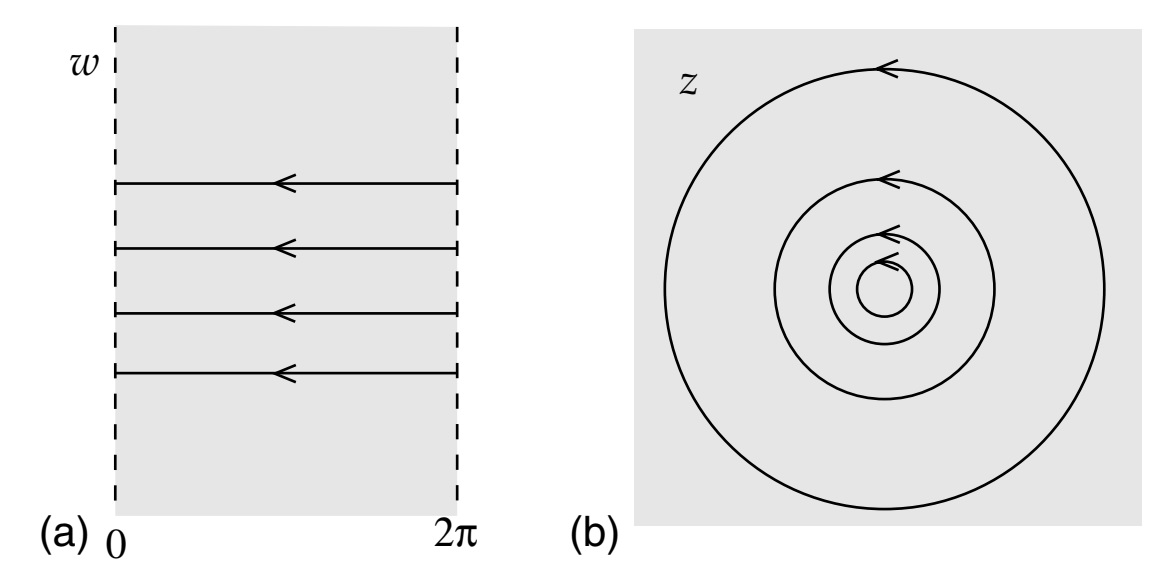
\includegraphics[width=0.8\textwidth]{figure/Fig2.3.jpg}
		\caption{Closed String Coordinates    }
	\end{center}
\end{figure}

In $w$ coordinates, time corresponds to moving $\sigma^{2}=\operatorname{Im} w$. In $z$ coordinates, time moves radially, and the origin is the distant past. These coordinates are related through a conformal transformation.    
For the canonical interpretation of the theory, $w$ coordinates are natural, but $z$ coordinates are also quite useful, and most expressions are written in this frame of reference.    

For holomorphic or anti-holomorphic operators, we can perform a Laurent expansion    
\begin{equation}
	T_{z z}(z)=\sum_{m=-\infty}^{\infty} \frac{L_{m}}{z^{m+2}}, \quad \tilde{T}_{\bar{z} \bar{z}}(\bar{z})=\sum_{m=-\infty}^{\infty} \frac{\tilde{L}_{m}}{\bar{z}^{m+2}} \label{2.6.5}
\end{equation}
The coefficients are called Virasoro generators.    
Given by contour integrals    
\begin{equation}\label{2.6.6}
	L_{m}=\oint_{C} \frac{\dif z}{2 \pi \mi z} \: z^{m+2} T_{z z}(z)
\end{equation}
where $C$ is any contour around the origin counterclockwise.    
At $\sigma^2=0$, the Laurent expansion is an ordinary Fourier transform    
\begin{subequations} \label{2.6.7}
	\begin{align}
		T_{w w}(w)&=-\sum_{m=-\infty}^{\infty} \exp (\mi m \sigma^{1}-m \sigma^{2}) T_{m}   \label{2.6.7a}\\
		T_{\bar{w} \bar{w}}(\bar{w})&=-\sum_{m=-\infty}^{\infty} \exp (-\mi m \sigma^{1}-m \sigma^{2}) \tilde{T}_{m} \label{2.6.7b}
	\end{align}
\end{subequations}
where    
\begin{equation}\label{2.6.8}
	T_{m}=L_{m}-\delta_{m, 0} \frac{c}{24} \:, \qquad \tilde{T}_{m}=\tilde{L}_{m}-\delta_{m, 0} \frac{\tilde{c}}{24} \:.
\end{equation}
The additional offset in $T_0$ comes from the non-tensor transformation (\ref{2.4.26})    
\begin{equation}
	T_{w w}=(\partial_{w} z)^{2} T_{z z}+\frac{c}{24} \:.
\end{equation}
In the $w=\sigma^{1}+\mi \sigma^{2}$ frame, the time-translation Hamiltonian is    
\begin{equation}\label{2.6.10}
	H= \int_{0}^{2 \pi} \frac{\dif \sigma^{1}}{2 \pi} \: T_{22}=L_{0}+\tilde{L}_{0}-\frac{c+\tilde{c}}{24} \:.
\end{equation}
Note the +2 in the Laurent expansion, which is canceled by the conformal transformation of $T$ in the Fourier transform. Similarly, the Laurent expansion of a holomorphic field with weight $h$ will contain $h$ in the exponent.    
Cut open the path integral on a circle where time $Im{w}=\ln |z|$ is constant. The Virasoro generators become operators in the usual sense. Because of holomorphicity, the integral (\ref{2.6.6}) is independent of $C$, so in particular, it is invariant under time translation. That is, they are conserved charges, charges associated with conformal invariance.    

\begin{figure}[!htbp]
	\begin{center}
		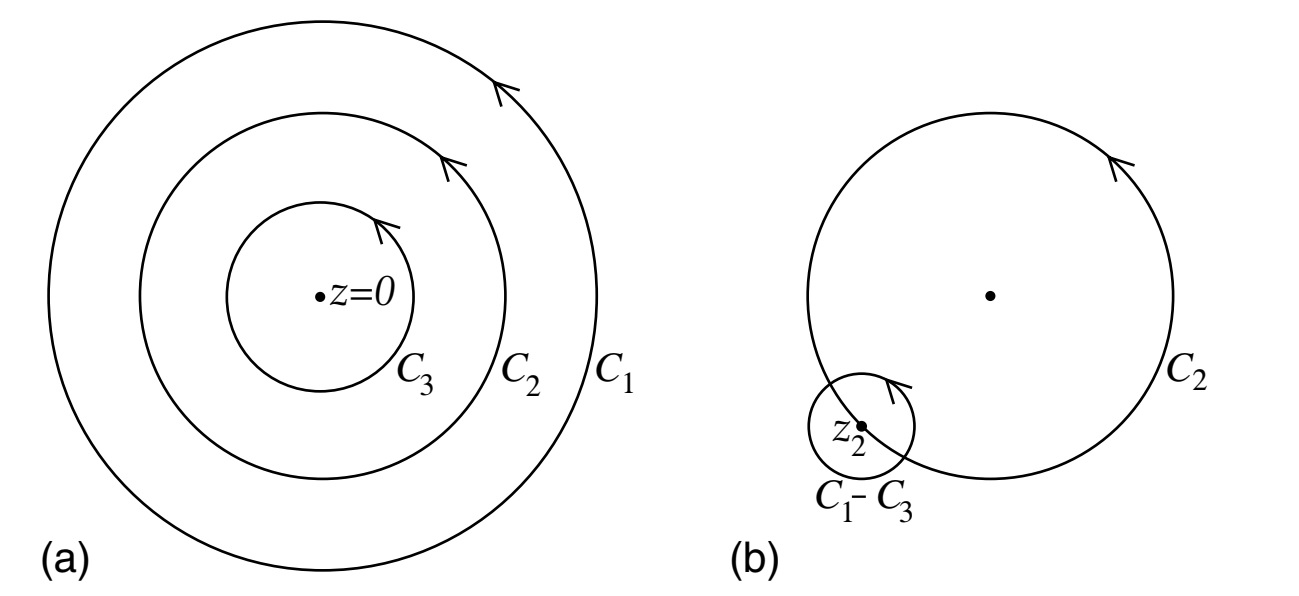
\includegraphics[width=0.6\textwidth]{figure/Fig2.4.jpg}
		\caption{Contours    }\label{Fig2.4}
	\end{center}
\end{figure}
An important fact: the OPE of currents determines the algebra of the corresponding charges.    
Examine general charges $Q_{i}, i=1,2$, given as contour integrals of holomorphic currents    
\begin{equation}
	Q_{i}\{C\}=\oint_{C} \frac{\dif z}{2 \pi \mi} j_{i}\label{2.6.11}
\end{equation}
Examine the combination    
\begin{equation}\label{2.6.12}
	Q_{1}\{C_{1}\} Q_{2}\{C_{2}\}- Q_{2}\{C_{2}\}Q_{1}\{C_{3}\}
\end{equation}
The contour is shown in Figure \ref{Fig2.4}a.    
\begin{figure}[!htbp]
	\begin{center}
		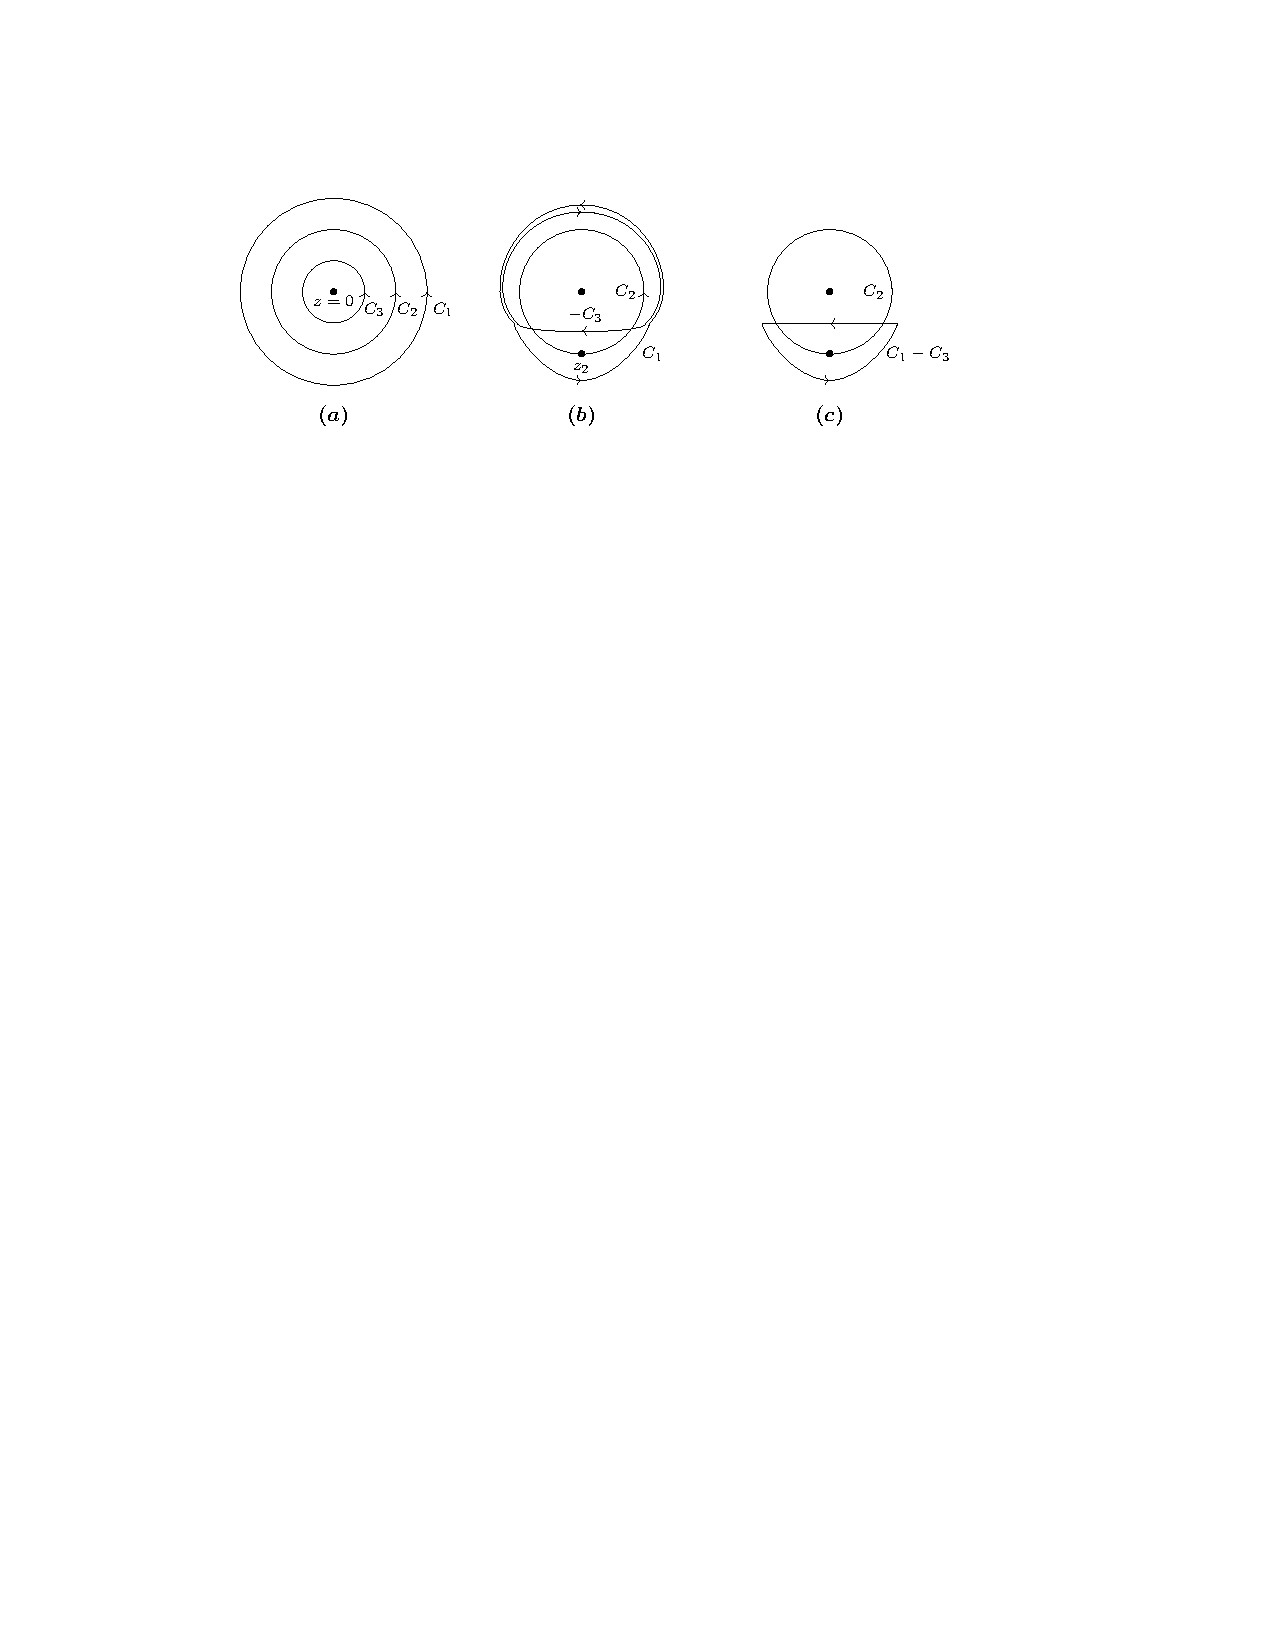
\includegraphics[width=0.8\textwidth]{figure/deforming contour}
		\caption{Deforming Contours. By deforming $C_3$ and $C_1$ is follows that $C_1 - C_3$ is equivalent to a contour around $z_2$.}
		\label{Fig2.4a}
	\end{center}
\end{figure}

The \textbf{order} of factors \textbf{is irrelevant} because they are just integration variables in a path integral (unless the two charges are anti-commuting. In that case there would be an extra sign and all commutators would become anti-commutators).    
When we split the path integral for an operator interpretation, the operator order is determined by time order, here $t_{1}>t_{2}>t_{3}$.    
The path integral for the combination (\ref{2.6.12}) corresponds to the matrix element    
\begin{equation}
	\hat{Q}_{1} \hat{Q}_{2}-\hat{Q}_{2} \hat{Q}_{1} \equiv [\hat{Q}_{1}, \hat{Q}_{2}]
\end{equation}
Now, for a given point $z_2$ on the contour $C_2$, we can deform the difference in contours $C_1, C_3$, as shown in Figure \ref{Fig2.4}b, so the commutator is given by the residue of the OPE    
\begin{equation}
	[Q_{1}, Q_{2}]\{C_{2}\}=\oint_{C_{2}} \frac{\dif z_{2}}{2 \pi \mi} \: \operatorname{Res}_{z_{1} \to z_{2}} j_{1}(z_{1}) j_{2}(z_{2}) \label{2.6.14}
\end{equation}
\begin{tcolorbox}[breakable]
	\begin{proof}
		We start from \eqref{2.6.12} but change the indices of the charges to letters to avoid confusion. It is the radial ordering of the contours that determines the \textbf{ordering} of the corresponding operators, therefore \( Q_a(C_1)Q_b(C_2) - Q_a(C_3)Q_b(C_2) \) object as operators on the Hilbert space is same as \( \hat{Q}_a\hat{Q}_b - \hat{Q}_b\hat{Q}_a = [\hat{Q}_a, \hat{Q}_b] \) as \( C_1 \) is the most outward contour, i.e. the largest time, and \( C_3 \) is the most inward contour, i.e. the smallest time. Now we also have
		\begin{equation}
			Q_a(C_1)Q_b(C_2) - Q_b(C_2)Q_a(C_3) = Q_b(C_2)[Q_a(C_1) - Q_a(C_3)]
			= Q_b(C_2)Q_a(C_1 - C_3)
		\end{equation}
		
		by the contour deformation of fig. \ref{Fig2.4a}. But, on the one hand the transformation of an operator is given by the commutation relation with the corresponding charge, \( \delta Q = [Q, A] \) and on the other hand we have from \eqref{2.3.11} that \( \delta A(z) = \frac{1}{2\pi i} \oint dw \, j(w)A(z) \) with \( j(z) \) the conserved current. Using a transformation under \( Q_a \) on an operator \( Q_b \) for a point on \( C_2 \) and the definition of the charges \eqref{2.6.11} we get
		\begin{align*}
			\delta Q_b\{C_2\} &= [Q_a, Q_b]\{C_2\} = Q_b(C_2)Q_a(C_1 - C_3)\\
			&=\oint_{C_2} \frac{dz_2}{2\pi i} \oint_{C_1-C_3} \frac{dz_1}{2\pi i} \, j_a(z_1)j_b(z_2)
		\end{align*}
		
		But the latter part just picks up the residue of the OPE \( j_a(z_1)j_b(z_2) \) when \( z_1 \to z_2 \). Thus
		
		\begin{equation}
			\delta Q_b\{C_2\} = \oint_{C_2} \frac{dz_2}{2\pi i} \, \operatorname{Res}_{z_1 \to z_2} j_a(z_1)j_b(z_2)
		\end{equation}
		
		and so we find
		
		\begin{equation}
			[\hat{Q}_a, \hat{Q}_b] = \oint_{C_2} \frac{dz_2}{2\pi i} \, \operatorname{Res}_{z_1 \to z_2} j_a(z_1)j_b(z_2)
		\end{equation}
		
		Which is the relation that allows us to pass from OPEs to the commutation relations of conserved charges.
	\end{proof}
\end{tcolorbox}
\begin{tcolorbox}[breakable]
	\begin{remark}
		The essential content of current--current OPEs is that charge commutators are determined by residues. If
		\begin{equation}
			J^a(z)\,J^b(w) \sim \frac{f^{ab}{}_c\, J^c(w)}{z-w} + \cdots,
		\end{equation}
		then defining
		\begin{equation}
			Q^a = \frac{1}{2\pi i}\oint dz\, J^a(z),
		\end{equation}
		we obtain
		\begin{equation}
			[Q^a, Q^b] = f^{ab}{}_c\, Q^c.
		\end{equation}
		Thus, the Lie algebra of charges is encoded in the simple pole of the current OPE.
	\end{remark}
\end{tcolorbox}
Contour discussion allows us to pass back and forth between OPEs and commutation relations.    
Let us emphasize that for conserved currents, knowing the singularity in the OPE is equivalent to knowing the corresponding charge commutator algebra. Replacing the conserved charge $Q_{2}\left\{C_{2}\right\}$ with an arbitrary operator, the same discussion applies:    
\begin{equation}
	[Q, \mathscr{A}(z_{2}, \bar{z}_{2})]=\operatorname{Res}_{z_{1} \to z_{2}} j(z_{1}) \mathscr{A}(z_{2}, \bar{z}_{2})
	=\frac{1}{\mi \epsilon} \delta \mathscr{A}(z_{2}, \bar{z}_{2}) \label{2.6.15}
\end{equation}
This is exactly the familiar statement: charge $Q$ generates the corresponding transformation. 
\begin{tcolorbox}[breakable]
\begin{remark}
	The symmetry action of $Q$ is encoded in the simple pole of the current--operator OPE:
	\begin{equation}
		j(z)\,\mathscr A(w,\bar w)
		\sim \frac{X(w,\bar w)}{z-w} + \cdots
		\;\Longrightarrow\;
		[Q,\mathscr A(w,\bar w)] = X(w,\bar w),
	\end{equation}
	with $\delta \mathscr A = i\epsilon\, X$. Placing the operator at the origin and using the state--operator correspondence
	\begin{equation}
		\mathscr A(0)\;\leftrightarrow\;|\mathscr A\rangle,
	\end{equation}
	this becomes
	\begin{equation}
		Q\,|\mathscr A\rangle = |X\rangle.
	\end{equation}
	Thus, the residue of the OPE determines both the transformation of operators and the action of the charge on states.
\end{remark}
\end{tcolorbox}   
Similarly, for contour integrals of anti-holomorphic currents    
\begin{equation}
	\tilde{Q}\{C\}=-\oint_{C} \frac{\dif \bar{z}}{2 \pi \mi} \: \tilde{\jmath} \:, \label{2.6.16}
\end{equation}
Ward identity and contour discussion imply    
\begin{equation}
	[\tilde{Q}, \mathscr{A}(z_{2}, \bar{z}_{2})]=\operatorname{Res}_{\bar{z}_{1} \to \bar{z}_{2}} \tilde{\jmath}(\bar{z}_{1}) 
	\mathscr{A}(z_{2}, \bar{z}_{2})=\frac{1}{\mi \epsilon} \delta \mathscr{A}(z_{2}, \bar{z}_{2}) \label{2.6.17}
\end{equation}
Applied to the Virasoro algebra (\ref{2.6.6}),    
\begin{align}
	&\operatorname{Res}_{z_{1} \to z_{2}} z_{1}^{m+1} T(z_{1}) z_{2}^{n+1} T(z_{2})  \nonumber \\
	&\quad =\operatorname{Res}_{z_{1} \rightarrow z_{2}} z_{1}^{m+1} z_{2}^{n+1}\Biggl(\frac{c}{2 z_{12}^{4}}+\frac{2}{z_{12}^{2}} T(z_{2})
	+\frac{1}{z_{12}} \partial T(z_{2})\Biggr) \nonumber \\
	&\quad =\frac{c}{12}(\partial^{3} z_{2}^{m+1}) z_{2}^{n+1}+2(\partial z_{2}^{m+1}) z_{2}^{n+1} T(z_{2})
	+z_{2}^{m+n+2} \partial T(z_{2}) \nonumber \\
	&\quad =\frac{c}{12}(m^{3}-m) z_{2}^{m+n-1}+(m-n) z_{2}^{m+n+1} T(z_{2})+\text {total derivative}  \label{2.6.18}
\end{align}
where $j_{m}(z)=z^{m+1} T(z)$.    
Then the $z_2$ contour integral on the right gives the Virasoro algebra:    
\begin{equation}\label{2.6.19}
	\left[L_{m}, L_{n}\right]=(m-n) L_{m+n}+\frac{c}{12}\left(m^{3}-m\right) \delta_{m,-n}
\end{equation}
$\tilde{L}_{m}$ satisfies the same algebra with central charge $\tilde{c}$.    
Thus any CFT has infinitely many conserved charges, i.e., Virasoro generators. They act in Hilbert space and satisfy algebra (\ref{2.6.19}). Focus on a few simple properties first. Generally, dealing with eigenstates of $L_{0}$ and $\tilde{L}_{0}$, generator $L_{0}$ satisfies    
\begin{equation}
	\left[L_{0}, L_{n}\right]=-n L_{n}
\end{equation}
If $|\psi\rangle$ is an eigenstate of $L_{0}$ with eigenvalue $h$, then    
\begin{equation}
	L_{0} L_{n}|\psi\rangle=L_{n}\left(L_{0}-n\right)|\psi\rangle=(h-n) L_{n}|\psi\rangle
\end{equation}
So $L_n|\psi\rangle$ is an eigenstate with eigenvalue $h-n$. Generators with $n<0$ raise the eigenvalue of $L_{0}$, while $n>0$ lowers it.    
Three generators $L_{0}$ , $L_{\pm 1}$ form a closed algebra without central charge:    
\begin{equation}
	\left[L_{0}, L_{1}\right]=-L_{1}, \quad\left[L_{0}, L_{-1}\right]=L_{-1}, \quad\left[L_{1}, L_{-1}\right]=2 L_{0}
\end{equation}
This is the algebra $SL(2,\mathbb{R})$, which differs from $SU(2)$ by a sign. For a holomorphic tensor field $\mathcal{O}$ with weight $(h,0)$, the Laurent coefficients are    
\begin{equation}
	\mathcal{O}(z)=\sum_{m=-\infty}^{\infty} \frac{_m}{z^{m+h}} \label{2.6.23}
\end{equation}
From OPE (\ref{2.4.16}) the commutator is obtained    
\begin{equation}
	[L_{m}, \mathcal{O}_{n}]=[(h-1) m-n] \mathcal{O}_{m+n} \:.
	\label{2.6.24}
\end{equation}
Again, $n>0$ mode lowers $L_0$, $n<0$ mode raises $L_0$.    

\begin{tcolorbox}[breakable]
	\begin{proof}
		Proof of (\ref{2.6.24}): in (\ref{2.6.17}) let $j_{m}(z)=z^{m+1} T(z)$ and $j_{n}(z)=z^{n+h-1} \mathcal{O}(z)$, then    
		\begin{align*}
			&\quad \operatorname{Res}_{z_1 \rightarrow z_2}  z_1^{m+1} T(z_{1}) z_2^{n+h-1} \mathcal{O}(z_{2})\\
			&=\operatorname{Res}_{z_1 \rightarrow z_2} z_1^{m+1} z_2^{n+h-1}\left(\frac{h}{z_{12}^2} O(z_2)+\frac{1}{z_{12}} \partial \mathcal{O}(z_2)\right)\\
			&=h(\partial z_2^{m+1})z_2^{n+h-1}\mathcal{O}(z_2)+z_2^{m+n+h}\partial\mathcal{O}(z_2)\\
			&=h(m+1)z_2^{m+n+h-1}\mathcal{O}(z_2)-(m+n+h)z_2^{m+n+h-1}\mathcal{O}(z_2)+ \text{total derivative}
		\end{align*}
		Using (\ref{2.6.23}), the first term becomes    
		$$h(m+1)z_2^{m+n+h-1}\mathcal{O}(z_2) \sim h(m+1) \sum \mathcal{O}_q z_2^{m+n-q-1} \sim h(m+1)\mathcal{O}_{m+n}$$
		The second term becomes    
		\begin{align*}
			-(m+n+h) z_{2}^{m+n+h-1} \sum \frac{\mathcal{O}_{q}}{z_{2}^{q+h}} \sim-(m+n+h) \mathcal{O}_{m+n}
		\end{align*}
		Adding the two yields (\ref{2.6.24}).    
	\end{proof}
\end{tcolorbox}

For open strings, let    
\begin{equation}
	0 \leq \operatorname{Re} w \leq \pi \quad \Leftrightarrow \quad \operatorname{Im} z \geq 0
\end{equation}
where $z=-\exp (-\mi w)$. 
The coordinate region is shown in Figure \ref{Fig2.5}.    
\begin{figure}[!htbp]
	\begin{center}
		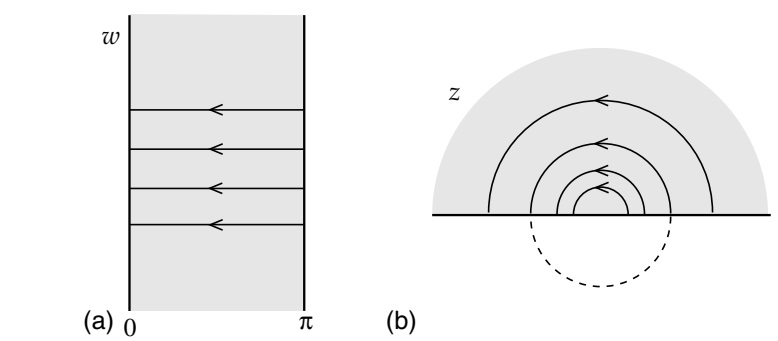
\includegraphics[width=0.8\textwidth]{figure/Fig2.5.jpg}
		\caption{Contours    }\label{Fig2.5}
	\end{center}
\end{figure}


\noindent At the boundary, energy-momentum satisfies    
\begin{equation}\label{2.6.26}
	T_{a b} n^{a} t^{b}=0 \:,
\end{equation}
where $n^{a}$ and $t^{b}$ are the normal vector and tangential vector respectively. To see this, examine a coordinate system where the boundary is a straight line. The appearance of the boundary breaks the normal translation invariance, but not the tangential one, making the current $T_{a b} t^{b}$ still conserved. Then the boundary condition (\ref{2.6.26}) is a statement that the current out of the boundary is zero.    
In the current case, this becomes    
\begin{equation}
	T_{w w}=T_{\bar{w} \bar{w}}, \: \operatorname{Re} w=0 \:, \pi \qquad \Leftrightarrow \quad T_{z z}=T_{\bar{z} \bar{z}}\:, \operatorname{Im} z=0 \:.
\end{equation}
It is convenient to use the "doubling trick".    
Define $T_{zz}$ in the lower half $z$-plane as the value of $T_{\bar{z} \bar{z}}$ at the image point $z^{\prime}=\bar{z}$ in the upper half plane:    
\begin{equation}
	T_{z z}(z) \equiv T_{\bar{z} \bar{z}}\left(\bar{z}^{\prime}\right), \quad \operatorname{Im} z<0 \:.
\end{equation}
Equations of motion and boundary conditions are summarized as: $T_{z z}$ is holomorphic throughout the complex plane.    
Because the boundary condition couples $T$ and $\tilde{T}$, there is only one set of Virasoro algebra:    
\begin{align}
	L_{m} &=\frac{1}{2 \pi \mi} \int_{C}\Bigl(\dif z \:z^{m+1} T_{z z}-\dif \bar{z} \: \bar{z}^{m+1} T_{\bar{z} \bar{z}}\Bigr) \nonumber  
	&=\frac{1}{2 \pi \mi} \oint \dif z\: z^{m+1} T_{z z}(z)
\end{align}
In the first line, the contour is a semicircle centered at the origin; in the second line, we use the "doubling trick" to write $L_m$ as a closed contour.    
Once again, these $L_{m}$ satisfy the Virasoro algebra    
\begin{equation}
	\left[L_{m}, L_{n}\right]=(m-n) L_{m+n}+\frac{c}{12}\left(m^{3}-m\right) \delta_{m,-n} \:.
\end{equation}

\section{\texorpdfstring{Mode expansions}{2.7 Mode expansions}} \label{sec:2.7}

\subsection*{Free Scalar}
In free field theory, the field decomposes into harmonic oscillators, and the spectrum and energy-momentum tensor can be given in mode form. We start with closed strings.    
In the theory of $X^\mu$, $\partial X$ and $\bar{\partial} X$ are anti-holomorphic. So there is a similar Laurent expansion:    
\begin{equation}\label{2.7.1}
	\partial X^{\mu}(z)=-\mi\biggl(\frac{\alpha^{\prime}}{2}\biggr)^{1 / 2} \sum_{m=-\infty}^{\infty} \frac{\alpha_{m}^{\mu}}{z^{m+1}}\:, \qquad 
	\bar{\partial} X^{\mu}(\bar{z})=-\mi\biggl(\frac{\alpha^{\prime}}{2}\biggr)^{1 / 2} \sum_{m=-\infty}^{\infty} \frac{\tilde{\alpha}_{m}^{\mu}}{\bar{z}^{m+1}} \:.
\end{equation}
Equivalently,    
\begin{subequations}\label{2.7.2}
	\begin{align}
		\alpha_{m}^{\mu}&=\biggl(\frac{2}{\alpha^{\prime}}\biggr)^{1 / 2} \oint \frac{\dif z}{2 \pi}\: z^{m} \partial X^{\mu}(z) \:, \label{2.7.2a} \\
		\tilde{\alpha}_{m}^{\mu}&=-\biggl(\frac{2}{\alpha^{\prime}}\biggr)^{1 / 2} \oint \frac{\dif \bar{z}}{2 \pi} \: \bar{z}^{m} \bar{\partial} X^{\mu}(\bar{z}) \:.
		\label{2.7.2b}
	\end{align}
\end{subequations}
The single-valuedness of $X^\mu$ implies $\alpha_{0}^{\mu}=\tilde{\alpha}_{0}^{\mu}$, furthermore, the Noether current of spacetime translation is $\mi \partial_{a} X^{\mu} / \alpha^{\prime}$, so spacetime momentum    
\begin{equation}\label{2.7.3}
	p^{\mu}=\frac{1}{2 \pi \mi} \oint_{C} (\dif z \: j^{\mu}-\dif \bar{z}\: \tilde{\jmath}^{\mu})
	=\biggl(\frac{2}{\alpha^{\prime}}\biggr)^{1 / 2} \alpha_{0}^{\mu}=\biggl(\frac{2}{\alpha^{\prime}}\biggr)^{1 / 2} \tilde{\alpha}_{0}^{\mu}
\end{equation}
Integrating expression (\ref{2.7.1}) gives    
\begin{equation}\label{2.7.4}
	X^{\mu}(z, \bar{z})=x^{\mu}- \mi \frac{\alpha^{\prime}}{2} p^{\mu} \ln |z|^{2}+\mi\left(\frac{\alpha^{\prime}}{2}\right)^{1 / 2} \sum_{m=-\infty \atop m \neq 0}^{\infty} \frac{1}{m}\left(\frac{\alpha_{m}^{\mu}}{z^{m}}+\frac{\tilde{\alpha}_{m}^{\mu}}{\bar{z}^{m}}\right) \:.
\end{equation}
Since $|z|>0$, the logarithm in mode decomposition does not have any branch cut. Whether starting from standard canonical commutators, or from contour discussions or the $XX$ OPE, one can give    
\begin{subequations} \label{2.7.5}
	\begin{align}
		[\alpha_{m}^{\mu}, \alpha_{n}^{\nu}] &= [\tilde{\alpha}_{m}^{\mu}, \tilde{\alpha}_{n}^{\nu}]=m \delta_{m,-n} \eta^{\mu \nu} \:, \label{2.7.5a} \\
		[x^{\mu}, p^{\nu}] &= \mi \eta^{\mu \nu} \:, \label{2.7.5b}  
	\end{align}
\end{subequations}
Other commutators are zero.    
The spectrum starts from the state $\lvert 0 ; k\rangle$ with momentum $k^\mu$, which is annihilated by all $n>0$ lowering modes $\alpha_n^\mu$, while other states in the spectrum are given by the action of raising modes $(n<0)$ in all possible ways on $\lvert 0 ; k\rangle$.    

We now wish to expand Virasoro generators in mode operator form.    
Substituting the Laurent expansion of $X^\mu$ into the energy-momentum tensor (\ref{2.4.4}) and collecting terms of a given order in $z$, gives    
\begin{equation}\label{2.7.6}
	L_{m} \sim \frac{1}{2} \sum_{n=-\infty}^{\infty} \alpha_{m-n}^{\mu} \alpha_{\mu n} \:.
\end{equation}
"$\sim$" means neglecting the order of operators. When $m\neq 0$, the expansion (\ref{2.7.6}) is well-defined and correct—the mode operator in each term commutes so the sequence is not important.    
For $m=0$, place the lowering operators on the right and introduce a normal-ordering constant:    
\begin{equation}
	L_{0}=\frac{\alpha^{\prime} p^{2}}{4}+\sum_{n=1}^{\infty}\left(\alpha_{-n}^{\mu} \alpha_{\mu n}\right)+a^{X} \:. \label{2.7.7}
\end{equation}
We encountered the same problem in Section 1.3, where we dealt with it in a heuristic way. Now there is a finite and explicit definition on the left, defined by Laurent coefficients in the $\mathrel{:\::}$ ordered energy-momentum tensor, so the normal-ordering constant is finite and calculable. There are several ways to determine it, the simplest is using the Virasoro algebra,    
\begin{equation}\label{2.7.8}
	2 L_{0}|0 ;
	0\rangle=(L_{1} L_{-1}-L_{-1} L_{1})|0 ; 0\rangle=0  \:,
\end{equation}
thus    
\begin{equation}
	a^{X}=0 \:. \label{2.7.9}
\end{equation}
Here we have used the known forms of $L_1, L_{-1}$: each term either contains a lowering operator or $p^\mu$, thus annihilating $|0 ; 0\rangle$.    
From the OPE, we determined the central charge of the Virasoro algebra. It can also be directly derived from the mode operator expression of the Virasoro algebra.    

Introduce a new notation. Symbol $ \mathrel{: \: :}$ represents creation-annihilation normal ordering: place all lowering operators on the right of all creation operators. Note there is a negative sign when exchanging anti-commuting operators.    
For this reason, we include $p^\mu$ among the lowering operators and $x^\mu$ among the raising operators.    
In this notation, we can write    
\begin{equation}\label{2.7.10}
	L_{m}=\frac{1}{2} \sum_{n=-\infty}^{\infty}\mathrel{ : \alpha_{m-n}^{\mu} \alpha_{\mu n} : }
\end{equation}


We have now introduced two forms of normal ordering, namely conformal normal ordering $\mathrel{:\::}$ and creation-annihilation normal ordering $\mathrel{: \: :}$. The advantage of the former is that the operators it produces have simpler OPEs and conformal transformation properties; the latter may be more familiar to readers, and it is more convenient for dealing with matrix elements of operators. We now present the relationship between the two. Start by comparing time-ordered products and creation-annihilation normal products.    
For the product $X^{\mu}(z, \bar{z}) X^{\nu}(z^{\prime}, \bar{z}^{\prime})$ with $\lvert z \rvert >\lvert z^{\prime}\rvert$, substitute in the mode expansion and move the lowering operator in $X^{\mu}(z, \bar{z})$ to the right:    
\begin{align}
	X^{\mu}(z, \bar{z}) X^{\nu}(z^{\prime}, \bar{z}^{\prime}) &= \mathrel{ : X^{\mu}(z, \bar{z}) X^{\nu}(z^{\prime}, \bar{z}^{\prime}) : }  +\frac{\alpha^{\prime}}{2} \eta^{\mu \nu}\left[-\ln |z|^{2}+\sum_{m=1}^{\infty} \frac{1}{m}\left(\frac{z^{\prime m}}{z^{m}}+\frac{\bar{z}^{\prime m}}{\bar{z}^{m}}\right)\right] \nonumber \\
	&=\mathrel{ : X^{\mu}(z, \bar{z}) X^{\nu}(z^{\prime}, \bar{z}^{\prime}) : }-\frac{\alpha^{\prime}}{2} \eta^{\mu \nu}\ln \lvert z-z^\prime\rvert^{2} \label{2.7.11}
\end{align}
Since $|z|>\lvert z^{\prime}\rvert$, the left side is time-ordered and the sum converges.    
Define the relationship between the time-ordered product and the conformal normal product given by (\ref{2.1.21}) (definition (\ref{2.1.21}) uses path integral language, so the products on the right are time-ordered under the operator system). This is the same as (\ref{2.7.11}), making    
\begin{equation}\label{2.7.12}
	\mathrel{ : X^{\mu}(z, \bar{z}) X^{\nu}(z^{\prime}, \bar{z}^{\prime}) : } = \mathrel{: X^{\mu}(z, \bar{z}) X^{\nu}(z^{\prime}, \bar{z}^{\prime})}:
\end{equation}
This relationship does not hold in a general CFT, and in fact, some combination of $p^\mu$ and lowering operators gives a simpler result. This also does not hold for the $w$ form of conformal normal sequence of operators.    
From (\ref{2.7.12}) the mode expansion (\ref{2.7.10}) can be written immediately, and the second derivation of $a^{X}=0$ is given.    

The creation-annihilation normal product of more than two $X^\mu$ has the same combinatorial factors as the $\mathrel{:\::}$ ordering. That is, they are both obtained from time-ordered products by summing over all contractions—Wick's theorem in field theory.    
To convert the normal ordering of an operator from one form to another, use the difference of two-point functions for contractions and sum over them. That is, if we have two orderings,    
\begin{equation}
	[X^{\mu}(z, \bar{z}) X^{v}(z^{\prime}, \bar{z}^{\prime})]_{1} = [X^{\mu}(z, \bar{z}) X^{v}(z^{\prime}, \bar{z}^{\prime})]_{2} 
	+\eta^{\mu v} \Delta (z, \bar{z}, z^{\prime}, \bar{z}^{\prime}) \:, \label{2.7.13}
\end{equation}
then for a general operator $\mathscr{F}$    
\begin{equation}
	[\mathscr{F}]_{1}=\exp \left(\frac{1}{2} \int \dif^{2} z\, \dif^{2} z^{\prime}\: \Delta(z, \bar{z}, z^{\prime}, \bar{z}^{\prime}) \frac{\delta}{\delta X^{\mu}(z, \bar{z})} \frac{\delta}{\delta X_{\mu}(z^{\prime}, \bar{z}^{\prime})}\right)[\mathscr{F}]_{2} \:.
	\label{2.7.14}
\end{equation}

For a linear dilaton CFT, the Laurent expansion and commutator are invariant, while the Virasoro generator contains an extra term    
\begin{equation}
	L_{m}=\frac{1}{2} \sum_{n=-\infty}^{\infty} \mathrel{ : \alpha_{m-n}^{\mu} \alpha_{\mu n} : } + \:\mi\left(\frac{\alpha^{\prime}}{2}\right)^{1 / 2}(m+1) V^{\mu} \alpha_{\mu m} \:.
\end{equation}

\subsection*{ $bc$ CFT}

Fields $b$ and $c$ have Laurent expansion    
\begin{equation} \label{2.7.16}
	b(z)=\sum_{m=-\infty}^{\infty} \frac{b_{m}}{z^{m+\lambda}}\:, \qquad c(z)=\sum_{m=-\infty}^{\infty} \frac{c_{m}}{z^{m+1-\lambda}} \:.
\end{equation}
Precisely, if $\lambda$ is an integer, they are just Laurent expansions. The half-integer case is also interesting, and we will deal with it carefully in Chapter 10. The OPE gives the anti-commutator    
\begin{equation}
	\left\{b_{m}, c_{n}\right\}=\delta_{m,-n} \:.
	\label{2.7.17}
\end{equation}
These operators anti-commute with other grassmann numbers as well. First examine states annihilated by all $n>0$ operators. The oscillator algebra of $b_0$ and $c_0$ generates two such ground states $\lvert\downarrow\rangle$ and $\lvert\uparrow\rangle$. They have properties    
\begin{subequations} \label{2.7.18}
	\begin{align}
		b_{0}\lvert\downarrow\rangle &=0\:, \quad b_{0} \lvert \uparrow\rangle=\lvert\downarrow\rangle \:, \label{2.7.18a} \\
		c_{0}\lvert\downarrow\rangle &=\lvert\uparrow\rangle \:, \quad c_{0}\lvert\uparrow\rangle=0 \:, \label{2.7.18b} \\
		b_{n}\lvert\downarrow\rangle &=b_{n}\lvert\uparrow\rangle=c_{n}\lvert \downarrow\rangle=c_{n}\lvert\uparrow\rangle=0 \:, \quad n>0  \:.
		\label{2.7.18c}
	\end{align}
\end{subequations}
Ordinary states are obtained by acting on these states with $n<0$ modes, but due to anti-commutation, they can act at most once. For some later reasons, it will be convenient to group $b_0$ with lowering operators and $c_0$ with raising operators, so we pick $\lvert \downarrow\rangle$ as the ghost vacuum $|0\rangle$. In string theory we will have a holomorphic $bc$ theory and an anti-holomorphic $\tilde{b} \tilde{c}$ theory. Each has $\lambda=2$.     
And the closed string spectrum contains the product of two pairs of theories.    
The Virasoro generators are    
\begin{equation}
	L_{m}=\sum_{n=-\infty}^{\infty}(m \lambda-n) \mathrel{ : b_{n} c_{m-n} : }+ \:\delta_{m, 0} a^{\mathrm{g}} \:.
	\label{2.7.19}
\end{equation}
The ordering constant can be determined like (\ref{2.7.8}), which gives    
\begin{align}
	2 L_{0}\lvert \downarrow\rangle &= (L_{1} L_{-1}-L_{-1} L_{1}) \lvert \downarrow\rangle \nonumber \\
	&= (\lambda b_{0} c_{1})[(1-\lambda) b_{-1} c_{0}]\lvert \downarrow\rangle=\lambda(1-\lambda)\lvert \downarrow\rangle \:.
	\label{2.7.20}
\end{align}
Thus $a^{\mathrm{g}}=\frac{1}{2} \lambda(1-\lambda)$ and    
\begin{equation}
	L_{m}=\sum_{n=-\infty}^{\infty}(m \lambda-n) \mathrel{ : b_{n} c_{m-n} : } + \: \frac{\lambda(1-\lambda)}{2} \delta_{m, 0} \:.
	\label{2.7.21}
\end{equation}
The constant can also be obtained by solving for the relationship between $\mathrel{:\::}$ and $\mathrel{: \: :}$.    
For the ghost number current (\ref{2.5.14}), $j={-}:\mathrel{bc}:$, the charge is    
\begin{align}
	N^{\mathrm{g}} &=-\frac{1}{2 \pi \mi} \int_{0}^{2 \pi} \dif w \: j_{w} \nonumber \\
	&=\sum_{n=1}^{\infty}(c_{-n} b_{n}-b_{-n} c_{n})+c_{0} b_{0}-\frac{1}{2} \:.
	\label{2.7.22}
\end{align}
It satisfies    
\begin{equation}
	[N^{\mathrm{g}}, b_{m}]=-b_{m}\:, \qquad  [N^{\mathrm{g}}, c_{m}]=c_{m} \:, \label{2.7.23}
\end{equation}
thus $c$ minus $b$ number is excitation. The ground states have ghost number $\pm \frac{1}{2}$:    
\begin{equation}
	N^{\mathrm{g}}\lvert \downarrow\rangle = -\frac{1}{2}\lvert \downarrow\rangle \:, \qquad 
	N^{\mathrm{g}}\lvert \uparrow\rangle = \frac{1}{2}\lvert \uparrow\rangle \:.
	\label{2.7.24}
\end{equation}
This depends on the value of the ordering constant, but can be guessed: the average ghost number of the ground state should be zero and the ghost number changes sign under $b \leftrightarrow c$.    

\subsection*{ Open String}
For open strings, Neumann boundary condition becomes $\partial_z X^{\mu}=\partial_{\bar{z}} X^{\mu}$ on the real axis.    
There is only one set of modes, the boundary condition requires $\alpha_{m}^{\mu}=\tilde{\alpha}_{m}^{\mu}$ in the expansion (\ref{2.7.1}).    
The spacetime momentum integral (\ref{2.7.3}) only integrates a semicircle, so the current normalization is    
\begin{equation}
	\alpha_{0}^{\mu}= (2 \alpha^{\prime})^{1 / 2} p^{\mu} \:. \label{2.7.25}
\end{equation}
Then the expansion for $X^\mu$ is    
\begin{equation}
	X^{\mu}(z, \bar{z})=x^{\mu}- \mi \alpha^{\prime} p^{\mu} \ln |z|^{2} + \mi\left(\frac{\alpha^{\prime}}{2}\right)^{1 / 2} 
	\sum_{m=-\infty \atop m \neq 0}^{\infty} \frac{\alpha_{m}^{\mu}}{m} (z^{-m}+\bar{z}^{-m}) \:.
	\label{2.7.26}
\end{equation}
Also    
\begin{equation}
	L_{0}=\alpha^{\prime} p^{2}+\sum_{n=1}^{\infty} \alpha_{-n}^{\mu}\cdot \alpha_{\mu n} \:. \label{2.7.27}
\end{equation}
Commutators as usual    
\begin{equation}
	[\alpha_{m}^{\mu}, \alpha_{n}^{\nu}]=m \delta_{m,-n} \eta^{\mu \nu} \: , \qquad [x^{\mu}, p^{\nu}]= \mi \eta^{\mu \nu} \:.
	\label{2.7.28}
\end{equation}

For $bc$ theory, the boundary conditions related to strings are    
\begin{equation}
	c(z)=\tilde{c}(\bar{z})\: , \quad b(z)=\tilde{b}(\bar{z}) \:, \quad \operatorname{Im} z=0 \:,  \label{2.7.29}
\end{equation}
which is the $z$ coordinate form where the boundary is on the real axis.    
Then we can use the doubling trick to write the holomorphic and anti-holomorphic fields in the upper half plane in the form of holomorphic fields in the entire plane    
\begin{equation}
	c(z) \equiv \tilde{c}(\bar{z}^{\prime})\:, \quad b(z) \equiv \tilde{b}(\bar{z}^{\prime})\:, \quad \operatorname{Im}(z) \leq 0\,,\: z^{\prime}=\bar{ z} \:.  \label{2.7.30}
\end{equation}
So for open strings, each $b$ and $c$ has a set of Laurent expansions.    
\section{\texorpdfstring{Vertex operators}{2.8 Vertex operators}}

In quantum field theory, on one hand, there is the state space of the theory; on the other hand, there is the set of local operators. In conformal field theory, there is a simple and useful isomorphism between them when quantizing the CFT on a circle.
Examine the semi-infinite cylinder in $w$-coordinates,    
\begin{equation}
	0 \leq \operatorname{Re} w \leq 2 \pi \:, \quad w \sim w+2 \pi \:, \quad \operatorname{Im} w \leq 0 \:, \label{2.8.1}
\end{equation}
under $z=\exp (-\mi w)$, this semi-infinite cylinder is mapped to a unit disk.    
As shown in Figure \ref{Fig2.6}.  Under this transformation, the entire $\sigma_2=-\infty$ hypersurface is mapped to the single point $z=0$. This naturally raises the question of whether any information has been lost. At first glance, it appears that the entire Hilbert space of the CFT is localized at a point in this coordinate system. If so, what structure encodes the seemingly lost information?

In a general QFT, this mapping is in fact singular: the metric $ds^2_{\rm cyl}$ becomes ill-defined at the origin, so one cannot meaningfully compress an entire hypersurface to a point. However, in a CFT, dilatation symmetry saves the situation. Since the states we consider form a basis of eigenstates of the dilatation operator, one can shrink any sphere to a point without losing information.

There is also a conceptual shift in locality. Operators defined on the $\sigma_2=-\infty$ hypersurface are intrinsically non-local objects from the radial point of view, whereas operators inserted at $z=0$ are genuine local operators. The information of the Hilbert space is therefore not lost, but reorganized and encoded in the space of local operator insertions at the origin, via the state--operator correspondence.
\begin{figure}[!htbp]
	\begin{center}
		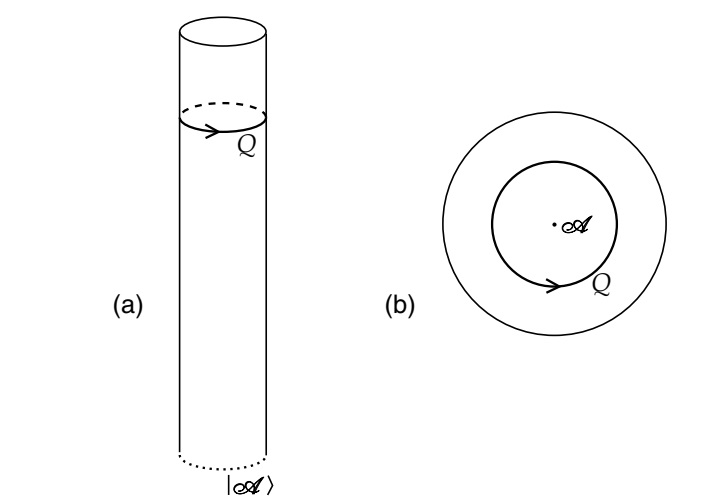
\includegraphics[width=0.8\textwidth]{figure/Fig2.6.jpg}
		\caption{(a) Semi-infinite cylinder in $w$-coordinates, with initial state $\lvert\mathscr{A}\rangle$ and charge $Q$. 
			(b) Conformal equivalent unit disk, with local operator $\mathscr{A}$ and contour integral of $Q$.    }\label{Fig2.6}
	\end{center}
\end{figure}

For free field theory, it is easy to get the detailed form of this isomorphism. Suppose there is a conserved charge $Q$ acting on state $\lvert\mathscr{A}\rangle$ as in Figure \ref{Fig2.6}(a). By using the OPE to calculate the contour integral in Figure \ref{Fig2.6}(b), the corresponding local operator can be found. Corresponding to the identity operator, we equate the state $|1\rangle$.    
When there is no operator at the origin, $\partial X^{\mu}$ and $\bar{\partial} X^{\mu}$ are holomorphic and anti-holomorphic inside the contour of $Q$ in Figure \ref{Fig2.6}(b). Define the contour integral (\ref{2.7.2}) of $\alpha_{m}^{\mu}$ and $\tilde{\alpha}_{m}^{\mu}$ for $m \geq 0$ to have no pole, thus yielding zero.    
$\lvert 1\rangle$ is annihilated by these modes, indicating it is the ground state,    
\begin{equation}
	\lvert 1\rangle=\lvert 0 ; 0\rangle \:, \label{2.8.2}
\end{equation}
now examine, for example, the state $\alpha_{-m}^{\mu}|1\rangle$ for positive $m$.    
Transitioning to Figure \ref{Fig2.6}(b), $Q=\alpha_{-m}^{\mu}$, the field is holomorphic within the contour, thus for $m\geq 1$ we get    
\begin{equation}\label{2.8.3}
	\alpha_{-m}^{\mu}=\left(\frac{2}{\alpha^{\prime}}\right)^{1 / 2} \oint \frac{\dif z}{2 \pi} \: z^{-m} \partial X^{\mu}(z) \rightarrow\left(\frac{2}{\alpha^{\prime}}\right)^{1 / 2} \frac{\mi}{(m-1) !} \partial^{m} X^{\mu}(0)
\end{equation}
so    
\begin{equation}
	\alpha_{-m}^{\mu}\lvert 1\rangle \cong\left(\frac{2}{\alpha^{\prime}}\right)^{1 / 2} \frac{\mi}{(m-1) !} \partial^{m} X^{\mu}(0)\:, \quad m \geq 1 \:.
	\label{2.8.4}
\end{equation}
Similarly    
\begin{equation}
	\tilde{\alpha}_{-m}^{\mu}|1\rangle \cong\left(\frac{2}{\alpha^{\prime}}\right)^{1 / 2} \frac{\mi}{(m-1) !} \bar{\partial}^{m} X^{\mu}(0)\:, \quad m \geq 1 \:. \label{2.8.5}
\end{equation}
When $\alpha_{-m}^{\mu}$ or $\tilde{\alpha}_{-m}^{\mu}$ act on general state $|\mathscr{A}\rangle$, this correspondence still holds.    
If $:\mathrel{ \mathscr{A}(0,0)}:$ is any normal-ordered operator, there may be singularities in the operator product of $\partial X^{\mu}(z)$ and $:\mathrel{ \mathscr{A}(0,0)}:$, 
but it is not hard to verify for $m>0$    
\begin{equation}
	\alpha_{-m}^{\mu} :\mathrel{\mathscr{A}(0,0)}:=:\mathrel{ \alpha_{-m}^{\mu} \mathscr{A}(0,0)}:  \:.
	\label{2.8.6}
\end{equation}
This is because the contour integral for this contraction will not have a simple singularity, then the same operation (\ref{2.8.3}) can be performed within the normal ordering, thus states with several $\alpha$ oscillator excitations appear as normal products $\mathrel{:\::}$ of corresponding operators    
\begin{subequations}\label{2.8.7}
	\begin{align}
		\alpha_{-m} &\rightarrow \mi\left(\frac{2}{\alpha^{\prime}}\right)^{1 / 2} \frac{1}{(m-1) !} \partial^{m} X^{\mu}(0)\:, \quad m \geq 1 \:,  \\
		\tilde{\alpha}_{-m}^{\mu} &\rightarrow \mi\left(\frac{2}{\alpha^{\prime}}\right)^{1 / 2} \frac{1}{(m-1) !} \bar{\partial}^{m} X^{\mu}(0)\:, \quad m \geq 1 \:,
	\end{align}
\end{subequations}
similarly    
\begin{equation}\label{2.8.8}
	x_{0}^{\mu} \rightarrow X^{\mu}(0,0) \:.
\end{equation}
Any operator can be obtained by acting with operators on the left of (\ref{2.8.7}) and (\ref{2.8.8}) on $|1\rangle$. 
The operator corresponding to that state is given by the normal product $\mathrel{:\::}$ of the corresponding local operator on the right. For example,    
\begin{equation}
	\lvert 0 ; k\rangle \cong \: : \mathrel{\me^{\mi k \cdot X(0,0)}}: \:.
	\label{2.8.9}
\end{equation}
This is easy to understand: under the translation $X^{\mu} \rightarrow X^{\mu}+a^{\mu}$, the state and the corresponding operator have the same translation, both being multiplied by $\me ^{\mi k\cdot a}$.     
\begin{tcolorbox}[breakable]
	One can show that
	\begin{equation*}
		\alpha_{m} \ket{0;k } = 0 \qquad \forall m > 0.
	\end{equation*}
	and
	\begin{align*}
		\hat{P}\ket{0;k}=k\ket{0;k}
	\end{align*}
	\noindent \textit{Proof.} By direct calculation:
	\begin{align*}
		\alpha_{m} \ket{0;k} &= \mi \sqrt{\frac{2}{\alpha^{\prime}}} \oint \frac{\dif z}{2 \pi \mi} z^{m} \partial X(z) \typecolon \sum_{n=0}^{\infty} \frac{(\mi k)^{n}}{n!} X^{n}(0) \typecolon \\
		&= \mi \sqrt{\frac{2}{\alpha^{\prime}}} \oint \frac{\dif z}{2 \pi \mi} z^{m} \left( - \frac{\mi k \alpha^{\prime}}{2} \frac{\typecolon \me^{\mi k X} \typecolon}{z} + \dots \right) \tag{using \eqref{ope: derivX-exp}}\\
		&= \sqrt{\frac{\alpha^{\prime}}{2}} k \operatorname{Res} \left[ z^{m} \frac{\typecolon \me^{\mi k X} \typecolon}{z} \right] \\
		&= 0 \qquad \forall m > 0.
	\end{align*}
	To show latter we utilize $[\hat{P},e^{ik\hat{X}}]=ke^{ik\hat{X}}$:
	\begin{align*}
		\hat{P}\ket{0;k} &=\hat{P}e^{ik\hat{X}}\ket{0;0}=e^{ik\hat{X}}\hat{P}\ket{0;0}+ke^{ik\hat{X}}\ket{0;0}\\
		&=k\ket{0;k}
	\end{align*}
\end{tcolorbox}
The same method applies to $bc$ theory. For clarity, we specify the case $\lambda=2$. This is of interest to bosonic string theory.    
From Laurent expansion and contour discussion gives    
\begin{equation}\label{2.8.10}
	b_{m}|1\rangle=0, \quad m \geq-1, \qquad c_{m}|1\rangle=0, \quad m \geq 2 \:.
\end{equation}
Note the shifts in the Laurent expansion exponents, which come from the conformal weights of $b$ and $c$. The identity operator is no longer mapped onto the ground state.    
Instead, relationship (\ref{2.8.11}) is determined    
\begin{equation}
	\lvert 1\rangle=b_{-1}\lvert \downarrow\rangle \:. \label{2.8.11}
\end{equation}
The translation of raising operators is straightforward,    
\begin{subequations} \label{2.8.12}
	\begin{align}
		b_{-m} &\rightarrow \frac{1}{(m-2) !} \partial^{m-2} b(0)\:, \quad m \geq 2 \:, \label{2.8.12a}  \\
		c_{-m} &\rightarrow \frac{1}{(m+1) !} \partial^{m+1} c(0)\:, \quad m \geq-1 \:.
		\label{2.8.12b}
	\end{align}
\end{subequations}
Note that the state $b_{-1}\lvert \downarrow\rangle$ with ghost number $-\frac{3}{2}$ is mapped onto the identity operator with ghost number 0, while the state $\lvert \downarrow\rangle$ with ghost number $-\frac{1}{2}$ is mapped onto the operator $c$ with ghost number 1. This difference comes from the non-tensor property (\ref{2.5.17}) of the ghost number current,    
\begin{equation}
	\partial_{z} w) j_{w}(w)=j_{z}(z)+q_{0} \frac{\partial_{z}^{2} w}{\partial_{z} w}=j_{z}(z)-\frac{q_{0}}{z} \:, \label{2.8.13}
\end{equation}
where $q_{0}=\lambda-\frac{1}{2}=\frac{3}{2}$.    
The expression for the cylindrical reference frame (\ref{2.7.22}) typically defines the ghost number of states, and the contour discussion in Figure \ref{Fig2.6} relates the ghost number of vertex operators with the polar coordinate system charge    
\begin{equation}
	Q^{\mathrm{g}} \equiv \frac{1}{2 \pi i} \oint \dif z\: j_{z}=N^{\mathrm{g}}+q_{0} \:.\label{2.8.14}
\end{equation}
This also applies to other charges: for tensor currents, the charge of the state and the corresponding operator are equal.    

Most of the above discussion can be extended to $\beta\gamma$ theory, but there are some difficulties under superstring.    

All concepts in this section can be extended to open strings.    
Half-infinite band    
\begin{equation}
	0 \leq \operatorname{Re} w \leq \pi, \quad \operatorname{Im} w \leq 0 \:, \label{2.8.15}
\end{equation}
is mapped to a semi-disk under $z=-\exp (-\mi w)$, i.e., the overlap region of the upper half plane and the unit circle.    
Initial state is again mapped to the origin, which is on the boundary, so there is an isomorphism    
\begin{equation}
	\text {local operator on the boundary } \leftrightarrow \text {state on the boundary} \:. \label{2.8.16}
\end{equation}
Details same as above. Doubling trick is useful in contour discussion.    

\subsection*{Path Integral Derivation}
Examine a disk in the $z$-plane, with local operator $\mathscr{A}$ at the origin, the field to be path integrated is $\phi$, this field takes fixed boundary value $\phi_{\mathrm{b}}$ on the unit circle.    
Path integrating over the internal field $\phi_i$ while keeping $\phi_{\mathrm{b}}$ constant gives the functional $\Psi_{\mathscr{A}}[\phi_{\mathrm{b}}]$,    
\begin{equation}
	\Psi_{\mathscr{A}}[\phi_{\mathrm{b}}]= \int[\dif  \phi_{\mathrm{i}}]_{\phi_{\mathrm{b}}} 
	\exp (-S[\phi_{\mathrm{i}}]) \mathscr{A}(0) \:. \label{2.8.17}
\end{equation}
The functional of fields is the Schrödinger representation of states, so this is the mapping from operators to states. The Schrödinger representation assigns a complex amplitude to each field configuration, with many uses.    

Alternatively, starting from some state $\Psi[\phi_{\mathrm{b}}]$. Examine path integration in the annular region $1 \geq |z|
\geq r$, 
where the field $\phi_{\mathrm{b}}$ on the outer circle is kept fixed, and path integrated over $\phi_{\mathrm{b}}^\prime$ along the inner circle as follows:    
\begin{equation}\label{2.8.18}
	\int [d \phi_{\mathrm{i}}]_{\phi_{\mathrm{b}}, \phi_{\mathrm{b}}^{\prime}} [\dif \phi_{\mathrm{b}}^{\prime}]\:
	\exp (-S[\phi_{\mathrm{i}}])\, r^{-L_{0}-\tilde{L}_{0}} \Psi[\phi_{\mathrm{b}}^{\prime}]
\end{equation}
that is, this integration is performed under weight $r^{-L_{0}-\tilde{L}_{0}} \Psi[\phi_{\mathrm{b}}^{\prime}]$.    
Now, 
path integration over the disk exactly corresponds to the propagation from $|z|=r$ to $|z|=1$, which is equivalent to acting with the operator $r^{+L_{0}+\tilde{L}_{0}}$. This cancels out the operator acting on $\Psi$, so (\ref{2.8.18}) is once again $\Psi[\phi_{\mathrm{b}}]$. 
\begin{tcolorbox}[breakable]			
			Let the outer radius be \(1\) and the inner radius be \(r<1\).  
			The Euclidean time \(\tau\) is related to the radial coordinate by \(|z|=e^{\tau}\);
			thus \(\tau_{\text{in}}=\ln r\) and \(\tau_{\text{out}}=0\).
			The Hamiltonian (dilatation generator) is \(H = L_0+\bar L_0\) (ignoring the central term).
			
		\begin{proof}
			Let the inner radius be $r$ and the outer radius $1$.  
			In radial quantization, time evolution from $r$ to $1$ is generated by $H = L_0+\bar L_0$:
			\[
			e^{-H(\tau_{\text{out}}-\tau_{\text{in}})} = e^{-H(0-\ln r)} = r^{H}.
			\]
			The path integral on the annulus with fixed boundary fields $\phi_b'$ (inner) and $\phi_b$ (outer) computes the matrix element
			\[
			\int [D\phi_i]_{\phi_b'\to\phi_b} e^{-S[\phi_i]} = \langle \phi_b | r^{H} | \phi_b' \rangle.
			\]
			Now take a state $|\psi_{\text{in}}\rangle$ on the inner circle, with wavefunctional $\psi_{\text{in}}(\phi_b') = \langle \phi_b' | \psi_{\text{in}} \rangle$.  
			Evolving it to the outer circle gives $|\psi_{\text{out}}\rangle = r^{H}|\psi_{\text{in}}\rangle$, whose wavefunctional is
			\[
			\psi_{\text{out}}(\phi_b) = \langle \phi_b | r^{H} | \psi_{\text{in}} \rangle
			= \int [D\phi_b'] \; \langle \phi_b | r^{H} | \phi_b' \rangle \; \langle \phi_b' | \psi_{\text{in}} \rangle.
			\]
			Substituting the path integral representation,
			\[
			\psi_{\text{out}}(\phi_b) = \int [D\phi_b'] [D\phi_i]_{\phi_b'\to\phi_b} e^{-S[\phi_i]} \; \psi_{\text{in}}(\phi_b').
			\]
			Identifying $\psi_{\text{out}}(\phi_b) = \Psi[\phi_b]$ and $\psi_{\text{in}}(\phi_b') =r^{-L_0-\bar L_0} \Psi[\phi_b']$ yields the desired equation.
		\end{proof}
\end{tcolorbox}
Now take the limit $r\to 0$. The annulus becomes a disk, and the limit of path integration over the inner circle can be considered as defining some local operator at the origin. According to this construction, path integration over the disk and this operator reproduce $\Psi[\phi_{\mathrm{b}}]$ on the boundary.    

We use a free scalar field $X$ as an example.    
Expanded on the unit circle    
\begin{equation}
	X_{\mathrm{b}}(\theta)=\sum_{n=-\infty}^{\infty} X_{n} \me^{\mi n \theta} \:, \quad X_{n}^{*}=X_{-n} \:. \label{2.8.19}
\end{equation}
The boundary state $\Psi[X_b]$ can be thought of as a function of all $X_n$.    
First identify the state corresponding to the identity operator, which is given by path integration without inserting any operators    
\begin{equation}
	\Psi_{1}[X_{\mathrm{b}}] = \int [\dif X_{\mathrm{i}}]_{X_{\mathrm{b}}} \exp \left(-\frac{1}{2 \pi \alpha^{\prime}} 
	\int \dif^{2} z\: \partial X \bar{\partial} X\right) \:. \label{2.8.20}
\end{equation}
Calculate it using the usual Gaussian method.    
Decompose $X_i$ into classical part and fluctuation    
\begin{subequations} \label{2.8.21}
	\begin{align}
		X_{\mathrm{i}}&=X_{\mathrm{cl}}+X_{\mathrm{i}}^{\prime} \:,\label{2.8.21a} \\
		X_{\mathrm{cl}}(z, \bar{z})&=X_{0}+\sum_{n=1}^{\infty}\left(z^{n} X_{n}+\bar{z}^{n} X_{-n}\right)  \:. \label{2.8.21b}
	\end{align}
\end{subequations}
Under this definition, $X_{\text{cl}}$ satisfies the equations of motion, $X_{\text{i}}^\prime$ is zero on the boundary.    
Then the path integral becomes    
\begin{equation}
	\Psi_{1}[X_{\mathrm{b}}]=\exp (-S_{\mathrm{cl}}) \int [\dif X_{\mathrm{i}}^{\prime}]_{X_{\mathrm{b}}=0} 
	\exp \left(-\frac{1}{2 \pi \alpha^{\prime}} \int \dif^{2} z\: \partial X^{\prime} \bar{\partial} X^{\prime}\right) \:,
	\label{2.8.22}
\end{equation}
where    
\begin{align}
	S_{\mathrm{cl}} &=\frac{1}{2 \pi \alpha^{\prime}} \sum_{m, n=1}^{\infty} m n X_{m} X_{-n} 
	\int_{|z|<1} \dif^{2} z\: z^{m-1} \bar{z}^{n-1}  \nonumber \\
	&=\frac{1}{\alpha^{\prime}} \sum_{m=1}^{\infty} m X_{m} X_{-m} \:.
	\label{2.8.23}
\end{align}
The integral over $X_i^\prime$ is a constant independent of boundary conditions, so    
\begin{equation}\label{2.8.24}
	\Psi_{1}[X_{\mathrm{b}}] \propto \exp \left(-\frac{1}{\alpha^{\prime}} \sum_{m=1}^{\infty} m X_{m} X_{-m}\right) \:.
\end{equation}
This is Gaussian type, actually the ground state.    
To see this, write raising and lowering operators in Schrödinger basis,    
\begin{subequations} \label{2.8.25}
	\begin{align}
		\alpha_{n}=-\frac{\mi n}{(2 \alpha^{\prime})^{1 / 2}} X_{-n}-\mi\left(\frac{\alpha^{\prime}}{2}\right)^{1 / 2} \frac{\partial}{\partial X_{n}} \:, \label{2.8.25a} \\
		\tilde{\alpha}_{n}=-\frac{\mi n}{(2 \alpha^{\prime})^{1 / 2}} X_{n}-\mi\left(\frac{\alpha^{\prime}}{2}\right)^{1 / 2} \frac{\partial}{\partial X_{-n}} \:, \label{2.8.25b} 
	\end{align}
\end{subequations} 
which comes from the Laurent expansion at $|z|=1$ and the mode algebra. Applying them on (\ref{2.8.24}), we find    
\begin{equation}
	\alpha_{n} \Psi_{1} [X_{\mathrm{b}}]=\tilde{\alpha}_{n} \Psi_{1}[X_{\mathrm{b}}]=0\:, \quad n \geq 0 \:, \label{2.8.26}
\end{equation}
so this is indeed the ground state. Therefore    
\begin{equation}
	|1\rangle \propto|0 ; 0\rangle \:. \label{2.8.27}
\end{equation}
We do not track the total normalization factor of the path integral, but define $|1\rangle =|0 ; 0\rangle$.    

Another simple calculation is the state corresponding to $\partial^{k} X$; this is just adding a factor $\partial^{k} X_{\mathrm{cl}}(0)=k ! X_{k}$ to existing result, so    
\begin{equation}
	\lvert \partial^{k} X \rangle=k ! X_{k} \Psi_{1}=-\mi\left(\frac{\alpha^{\prime}}{2}\right)^{1 / 2}(k-1) !
	\alpha_{-k}|0 ; 0\rangle \:, \label{2.8.28}
\end{equation}
similar for $\bar{\partial}^{k} X$. This can be generalized to all products of derivatives and exponentials of $X$. Conformal normal ordering only cancels out effect of $X_\mathrm{i}^\prime$ path integral.    

\section{\texorpdfstring{More on states and operators}{2.9 More on states and operators}} \label{sec:2.9}

\subsection*{OPE}
In this section we make some other applications of the state-operator correspondence. The first is a general extension of the OPE, as shown in Figure \ref{Fig2.7}.    
\begin{figure}[!htbp]
	\begin{center}
		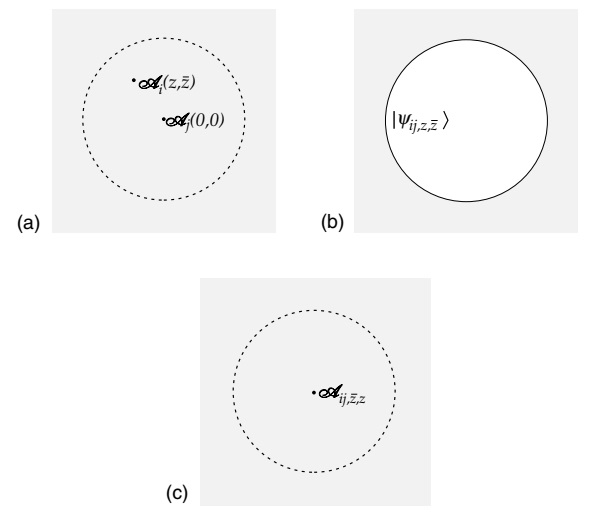
\includegraphics[width=0.8\textwidth]{figure/Fig2.7.jpg}
		\caption{(a) Worldsheet with two local operators. (b) Integrating over fields inside the disk gives boundary state $\lvert\psi_{i j, z, \bar{z}}\rangle$. (c) Cutout inside a disk with corresponding local operators. Expanding to operators with definite weights gives OPE.    }\label{Fig2.7}
	\end{center}
\end{figure}
Examine product    
\begin{equation}
	\mathscr{A}_{i}(z, \bar{z}) \mathscr{A}_{j}(0,0) \:, \label{2.9.1}
\end{equation}
where $|z|<1$. We can split the path integral into integration over field $\phi_{\mathrm{i}}$ inside unit circle, field $\phi_{\mathrm{b}}$ on unit circle, field $\phi_{\mathrm{e}}$ outside unit circle.    
As discussed at the end of last section, integration over $\phi_{\mathrm{i}}$ yields some functional of $\phi_{\mathrm{b}}$, denoted as $\Psi_{i j, z, \bar{z}}[\phi_{\mathrm{b}}]$. Via state--operator correspondence, this is equivalent to gluing disk together with appropriate operator $\mathscr{A}$. To turn it into standard form expanded with complete set of $L_{0}, \tilde{L}_{0}$ eigenstates    
\begin{equation}
	\mathscr{A}_{i j, z, \bar{z}}=\sum_{k} z^{h_{k}-h_{i}-h_{j}}\bar{z}^{\tilde{h}_{k}-\tilde{h}_{i}-\tilde{h}_{j} }c^{k}{}_{i j} \mathscr{A}_{k} \:, \label{2.9.2}
\end{equation}
where $z$ dependence and $\bar{z}$ dependence are determined by conformal weights like (\ref{2.4.20}).   
\begin{tcolorbox}[breakable]
\begin{proof} 
We consider the product of two operators acting on the vacuum. In radial quantization, $\mathcal{A}_j(0,0)$ creates a state at the origin, and $\mathcal{A}_i(z,\bar{z})$ acts as an operator on the Hilbert space at radius $|z|$.
\begin{equation}
	|\Psi_{ij}(z,\bar{z})\rangle = \mathcal{A}_i(z,\bar{z}) \mathcal{A}_j(0,0) |0\rangle = \mathcal{A}_i(z,\bar{z}) |\mathcal{A}_j\rangle
\end{equation}
Since $\{|\mathcal{A}_k\rangle = \mathcal{A}_k(0,0)|0\rangle\}$ forms a complete basis for the Hilbert space, we expand the state $|\Psi\rangle$:
\begin{equation}
	|\Psi_{ij}(z,\bar{z})\rangle = \sum_k C_{ij}^k(z,\bar{z}) |\mathcal{A}_k\rangle
\end{equation}
To find the $z$-dependence, we apply the dilatation generator $L_0$. For a primary operator $\mathcal{A}_i$ with weight $h_i$, the commutator is:
\begin{equation}
	[L_0, \mathcal{A}_i(z,\bar{z})] = (z \partial_z + h_i) \mathcal{A}_i(z,\bar{z})
\end{equation}
Applying $L_0$ to the state $|\Psi_{ij}\rangle$ and using $L_0 |\mathcal{A}_j\rangle = h_j |\mathcal{A}_j\rangle$:
\begin{align}
	L_0 |\Psi_{ij}(z,\bar{z})\rangle &= L_0 \mathcal{A}_i(z,\bar{z}) |\mathcal{A}_j\rangle \notag\\
	&= [L_0, \mathcal{A}_i(z,\bar{z})] |\mathcal{A}_j\rangle + \mathcal{A}_i(z,\bar{z}) L_0 |\mathcal{A}_j\rangle\notag \\
	&= (z \partial_z + h_i + h_j) |\Psi(z,\bar{z})\rangle
\end{align}

Applying $L_0$ to the basis expansion side:
\begin{equation}
	L_0 \sum_k C_{ij}^k(z,\bar{z}) |\mathcal{A}_k\rangle = \sum_k h_k C_{ij}^k(z,\bar{z}) |\mathcal{A}_k\rangle
\end{equation}
Equating both sides, the coefficients $C_{ij}^k$ must satisfy:
\begin{equation}
	(z \partial_z + h_i + h_j) C_{ij}^k(z,\bar{z}) = h_k C_{ij}^k(z,\bar{z})
\end{equation}
Rearranging gives the scaling equation:
\begin{equation}
	z \partial_z C_{ij}^k = (h_k - h_i - h_j) C_{ij}^k
\end{equation}
The solution is:
\begin{equation}
	C_{ij}^k(z,\bar{z}) = c_{ij}^k z^{h_k - h_i - h_j} \bar{z}^{\bar{h}_k - \bar{h}_i - \bar{h}_j}
\end{equation}

Stripping the vacuum state, we recover the OPE in its standard form:
\begin{equation}
	\mathcal{A}_i(z,\bar{z}) \mathcal{A}_j(0,0) = \sum_k c_{ij}^k z^{h_k - h_i - h_j} \bar{z}^{\bar{h}_k - \bar{h}_i - \bar{h}_j} \mathcal{A}_k(0,0)
\end{equation}
	QED.
\end{proof}
\end{tcolorbox} 
Convergence of OPE is exactly convergence of a complete set in quantum mechanics. As long as there is no other operator in $\lvert z^{\prime}\rvert \leq \lvert z\rvert$, this construction is possible. Allowing us to cut out circle of radius $|z|+\epsilon$.    
For three operators    
\begin{equation}
	\mathscr{A}_{i}(0,0) \mathscr{A}_{j}(1,1) \mathscr{A}_{k}(z, \bar{z}) \:, \label{2.9.3}
\end{equation}
convergence region $|z|<1$ of $z\to 0$ OPE overlaps with convergence region $|1-z|<1$ of $z\to 1$ OPE. Then coefficient of $\mathscr{A}_l$ in triple product can be written as summation including $c^{l}{}_{i k} c^{m}{}_{l j}$ or summation including $c^{l}{}_{j k} c^{m}{}_{li}$. Associativity requires these sums to be equal.    
Graphic representation see Figure \ref{Fig2.8}.    
\begin{figure}[!htbp]
	\begin{center}
		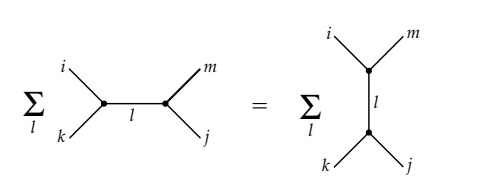
\includegraphics[width=0.8\textwidth]{figure/Fig2.8.jpg}
		\caption{Graphical representation of OPE associativity    }\label{Fig2.8}
	\end{center}
\end{figure}

\subsection*{Virasoro Algebra and Highest Weight States}

Now apply discussion in Figure \ref{Fig2.6} to Virasoro generators:    
\begin{align}
	L_{m}\lvert \mathscr{A}\rangle & \cong \oint \frac{\dif z}{2 \pi \mi}\: z^{m+1} T(z) \mathscr{A}(0,0)  \nonumber \\
	& \cong L_{m} \cdot \mathscr{A}(0,0) \:.
	\label{2.9.4}
\end{align}
Here we entered new notation and concept. Given state-operator isomorphism, each operator acting on Hilbert space has an image acting on local operator space. In other words, formed corresponding contour around operator and calculated corresponding local operator using OPE. Corresponding to $L_m$ mapping states to states is $L_m\cdot$ mapping local operators to local operators. Generally there will be local operators at different positions $z_i$, and each position will have a different version of Virasoro algebra. These different versions are obtained by Laurent expansion centered at operator position. A standard basis for generators will also exist in some geometries.    
For example for cylinder then expansion centered at $z=0$. "$\cdot$" acts as a reminder: what we discuss is Laurent expansion coefficient around specific operator.    

In this notation, $T\mathscr{A}$ OPE is    
\begin{equation}\label{2.9.5}
	T(z) \mathscr{A}(0,0)=\sum_{m=-\infty}^{\infty} z^{-m-2} L_{m} \cdot \mathscr{A}(0,0) \:.
\end{equation}
To relate to earlier notation (\ref{2.4.11}), for $n \geq 0$, $\mathscr{A}^{(n)}=L_{n-1} \cdot \mathscr{A}$, conformal transformation of $\mathscr{A}$ is    
\begin{equation}
	\delta \mathscr{A}(z, \bar{z})=-\epsilon \sum_{n=0}^{\infty} \frac{1}{n !}\Bigl[\partial^{n} v(z) L_{n-1}+\left(\partial^{n} v(z)\right)^{*} \tilde{L}_{n-1}\Bigr] \cdot \mathscr{A}(z, \bar{z}) \:.
	\label{2.9.6}
\end{equation}
Using general form of $T\mathscr{A}$ OPE (\ref{2.4.14}), we have very useful results    
\begin{subequations}\label{2.9.7}
	\begin{align}
		L_{-1} \cdot \mathscr{A}&=\partial \mathscr{A}, \quad \tilde{L}_{-1} \cdot \mathscr{A}=\bar{\partial} \mathscr{A} \:, \label{2.9.7a} \\
		L_{0} \cdot \mathscr{A}&=h \mathscr{A}, \quad \tilde{L}_{0} \cdot \mathscr{A}=\tilde{h} \mathscr{A} \:.\label{2.9.7b}
	\end{align}
\end{subequations}
OPE (\ref{2.9.5}) implies state corresponding to primary field $\mathcal{O}$ with weight $(h, \tilde{h})$ satisfies    
\begin{subequations} \label{2.9.8}
	\begin{align}
		L_{0}|\mathcal{O}\rangle&=h|\mathcal{O}\rangle \:, \quad \tilde{L}_{0}|\mathcal{O}\rangle=\tilde{h}|\mathcal{O}\rangle \:, \label{2.9.8a} \\
		L_{m}|\mathcal{O}\rangle&=\tilde{L}_{m}|\mathcal{O}\rangle=0\:, \quad m>0 \:.
		\label{2.9.8b}
	\end{align}
\end{subequations}
Such state is called highest weight state: by repeatedly acting with lowering operators on arbitrary state, we eventually obtain state annihilated by further lowering operators, called highest weight state.    

An interesting special case is identity operator, operator product $T1$ is non-singular, so in arbitrary CFT get    
\begin{equation}
	L_{m}|1\rangle=\tilde{L}_{m}|1\rangle=0, \quad m \geq-1 \:.
	\label{2.9.9}
\end{equation}
As marked in 2.4, operators $L_{0}$ and $L_{\pm 1}$ form closed algebra, so do $\tilde{L}_{0}$ and $\tilde{L}_{\pm 1}$. Entire algebra is    
\begin{equation}
	SL(2,\mathds{R})\times SL(2,\mathds{R})= S L(2, \mathds{C}) \:. \label{2.9.10}
\end{equation}
Therefore $|1\rangle$ is also called $SL(2, \mathds{C})$-invariant state.    
It is the only such state, because (\ref{2.9.7}) implies any operator $\mathscr{A}$ corresponding to $SL(2, \mathds{C})$-invariant state is independent of position, so must be $c$-number, as explained after (\ref{2.4.24}).    

\subsection*{Unitary CFT}

Highest weight states play important role in string theory and representation theory of Virasoro algebra. Now we derive several important results generally valid in unitary CFT.    
Unitary CFT has positive definite inner product, making    
\begin{equation}
	L_{m}^{\dagger}=L_{-m} \: , \quad \tilde{L}_{m}^{\dagger}=\tilde{L}_{-m} \:. \label{2.9.11}
\end{equation}
Recall: inner product via $\langle\alpha \vert A \beta\rangle=\langle A^{\dagger} \alpha \vert \beta\rangle$ defined adjoint.    
For example $X^\mu$ CFT for \emph{spacelike} $\mu$ is unitary. If we take inner product of ground states as    
\begin{equation}
	\langle 0 ; k \vert 0 ;
	k^{\prime} \rangle=2 \pi \delta(k-k^{\prime})  \label{2.9.12}
\end{equation} 
and define    
\begin{equation}
	\alpha_{m}^{\dagger}=\alpha_{-m} \:, \quad \tilde{\alpha}_{m}^{\dagger}=\tilde{\alpha}_{-m} \:. \label{2.9.13}
\end{equation}
This implicitly defines inner product of all higher states. This CFT for $X^\mu=0$ is not unitary, because there is negative sign in commutation relation there.    

First constraint in unitary CFT is any state must have $h, \tilde{h} \geq 0$.    
If this holds for highest weight states, then it holds for all states. For highest weight states, Virasoro algebra gives    
\begin{equation}\label{2.9.14}
	2 h_{\mathcal{O}}\langle\mathcal{O} \vert \mathcal{O}\rangle=2\langle\mathcal{O}\vert L_{0}\vert \mathcal{O}\rangle=\langle\mathcal{O}|[L_{1}, L_{-1}]|\mathcal{O}\rangle=\| L_{-1}|\mathcal{O}\rangle \|^{2} \geq 0 \:,
\end{equation}
so $h_{\mathcal{O}} \geq 0 $.    
If $h_{\mathcal{O}}=\tilde{h}_{\mathcal{O}}=0$, then    
\begin{equation}
	L_{-1} \cdot \mathcal{O}=\tilde{L}_{-1} \cdot \mathcal{O}=0 \:, \label{2.9.15}
\end{equation}
thus $\mathcal{O}$ is independent of position. As previously marked, $\mathcal{O}$ must be $c$-number, i.e., in unitary CFT identity operator is unique $(0,0)$ operator. Surprisingly, $X^\mu$ is unique exception: corresponding state $x^{\mu}|0 ;
0\rangle$ is non-normalizable due to infinite range of $X^\mu$, and equation (\ref{2.9.14}) no longer holds.    
For CFT corresponding to compact dimension, general theorem is most useful, such exceptions cannot occur.    

In same way, in unitary CFT, if and only if $\tilde{h}=0$, operator is holomorphic, and if and only if $h=0$, operator is anti-holomorphic;    
this is an important result, repeated as follows:    
\begin{equation}
	\partial \mathscr{A}=0 \Leftrightarrow h=0 \:, \quad \bar{\partial} \mathscr{A}=0 \Leftrightarrow \tilde{h}=0 \:. \label{2.9.16}
\end{equation}
Finally, using previous discussion and commutator $\left[L_{n}, L_{-n}\right]$ it can be proven that in unitary CFT $c, \tilde{c} \geq 0$.    
Actually, unique unitary CFT with $c=0$ is trivial: $L_n=0$.    

\subsection*{Zero-point energy}
State-operator mapping gives another simple derivation of different normal-ordering constants. In any CFT, we know $L_{0}|1\rangle=0$, and this determines another normalization of $L_0$.    
In $X$ CFT, $|1\rangle=0$ is ground state, so $a^X=0$.    
In $bc$ theory, $|1\rangle=0$ is excited state $b_{-1}\lvert \downarrow\rangle$, so to be consistent with earlier $\lambda=2$ result (\ref{2.7.1}), weight of $\lvert \downarrow\rangle$ is $-1$.    

This also provides physical interpretation of central charge. In unitary CFT, ground state is $|1\rangle$ with $L_{0}=\tilde{L}_{0}=0$.    
Conformal transformation (\ref{2.6.10}) between radial generator and time translation generator implies for ground state    
\begin{equation}
	E=-\frac{c+\tilde{c}}{24} \:.
	\label{2.9.17}
\end{equation}
This is Casimir energy, arising from finite scale of system, and dependent on central charge. Based on dimensional analysis, this energy is inversely proportional to size $\ell$ of system, here $2\pi$, so general result is    
\begin{equation}
	E=-\frac{\pi(c+\tilde{c})}{12 \ell} \:. \label{2.9.18}
\end{equation}
We now have three ways to calculate normal-ordering constants:    
\begin{enumerate}
	\item Like in (\ref{2.7.8}), starting from Virasoro algebra;
	\item Like in (\ref{2.7.11}), relating two forms of normal ordering;
	\item Starting from previous state-operator mapping.    
\end{enumerate}
However method of adding up zero-point energy is intuitive, so we give another description:    
\begin{enumerate}
	\item For each boson mode, zero-point energy is $\frac{1}{2} \omega$; for each fermion mode, zero-point energy is $-\frac{1}{2} \omega$. Add up energy.
	\item Encountering divergent sum of form $\sum_{n=1}^{\infty}(n-\theta)$, where $\theta$ comes from non-trivial periodicity conditions, define it as    
	\begin{equation}
		\sum_{n=1}^{\infty}(n-\theta)=\frac{1}{24}-\frac{1}{8}(2 \theta-1)^{2} \:. \label{2.9.19}
	\end{equation}
	This value can be obtained, as in \eqref{1.3.32}, by regularizing and discarding the quadratically divergent part. 
	\item The normal ordering constant for the generator $T_0$ in the $w$ frame was provided earlier, where $T_0$ is defined by (\ref{2.6.8}). 
	For $L_0$, we must add the non-tensor correction $\frac{1}{24} c$. 
\end{enumerate}
For the free bosonic field, the modes are integer-valued; thus, after step 2, for $\theta=0$, we obtain half of the sum, which is $-\frac{1}{24}$.  This is exactly canceled by the correction in step 3, giving $a^X=0$.  For the ghost fields, we similarly obtain $\frac{2}{24}-\frac{26}{24}=-1$.